% Preserve TeX's year register: the IEEE Access class defines a conflicting year setter.
\let\BAREprimitiveyear\year
\documentclass[nolineno]{ieeeaccess}
\let\year\BAREprimitiveyear
\renewcommand{\theyear}{2026}
\vol{Draft}
\usepackage{cite,amsmath,amssymb,graphicx,booktabs,tabularx,array}
\usepackage{algorithm,algpseudocode}
\usepackage{tikz}\usetikzlibrary{arrows.meta,positioning}
% RGB fallback avoids incompatible spot-color definitions when TikZ loads xcolor.
\definecolor{accessblue}{RGB}{0,103,143}
\usepackage[hidelinks]{hyperref}
\newcommand{\sg}{\operatorname{stopgrad}}
\newcommand{\MAE}{\operatorname{MAE}}
\newcommand{\softmax}{\operatorname{softmax}}
\setlength{\emergencystretch}{1em}
\begin{document}
\history{Experimental research draft. Run date: 30 September 2026. Not accepted or published.}
\doi{}
\title{BARE: Budgeted Regional Evidence Acquisition with Gradient-Replayed Training for Bone Age Estimation on a 4 GB GPU}
\author{}
\address{}
\corresp{}
\markboth{BARE: Research Draft}{BARE: Research Draft}
\begin{abstract}
High-resolution multiview bone age models can be difficult to train under a laptop video-memory constraint. This paper presents the implementation of Budgeted Acquisition of Regional Evidence, which combines a shared MobileNetV3-Large encoder, small evidence-set attention, ordinal age-distribution learning, model-defined crop-utility supervision and deterministic token-gradient replay. This version reports preliminary executed results from global warmup and completed resource/correctness experiments; full multiview acquisition training is still running. A frozen early global checkpoint achieved 8.285 months mean absolute error and 10.928 months root mean squared error on 1259 development images. These model-selection results are not independent test performance. A ten-view training admission profile measured 260 MiB reserved memory with replay versus 704 MiB with joint backpropagation, while both configurations fitted the four-gigabyte RTX 3050. A deterministic gradient test obtained relative error of approximately $4.54\times10^{-8}$. Results include development subgroups, fitting-only age-prior comparisons, optimization logs, software checks, resource measurements and five predetermined regression Grad-CAM cases. Forty verified references, a focused literature survey and protocol-qualified published accuracy/resource comparisons accompany the analysis. The official validation holdout remains unevaluated. The reported scope does not establish final acquisition accuracy, official-test state of the art, external generalization or clinical validity.
\end{abstract}
\begin{keywords}Bone age estimation, counterfactual utility, gradient replay, medical image analysis, memory-constrained learning, regional evidence acquisition.\end{keywords}
\titlepgskip=-15pt
\maketitle

\section{Introduction}
\PARstart{P}{ediatric} bone age estimation uses skeletal appearance in hand radiographs as a developmental indicator. Public benchmarks accelerated convolutional approaches, but their evaluation protocols and use of auxiliary annotations vary~\cite{halabi,larson,spampinato,lee,iglovikov,bonexpert}. The RSNA challenge separates 12,611 training, 1,425 validation and 200 test images~\cite{halabi}. A method evaluated on the public validation labels cannot be ranked directly against methods evaluated on the smaller official test set.

Attention-guided localization, local/global fusion and distribution learning are established bone-age techniques~\cite{chen,cfjl,selfsupervised,rfga,bonet,bogff,bonetplus,integral}. Regional CNNs can also be designed for lightweight operation~\cite{lightweight}. BARE investigates a narrower question: can the expected \emph{incremental} value of a crop be learned without encoding that unseen crop at inference, while preserving detailed regional supervision under a laptop memory budget?

Our implementation contributes three testable elements. First, it supervises crop utility with the change in model absolute error caused by adding a crop to a sampled evidence subset. Second, a small evidence-set model combines ordinal age learning with local descriptors, recorded sex, and regional disagreement. Third, replay separates fusion differentiation from encoder backpropagation, applying the existing gradient-caching principle~\cite{gradcache} to shared multiview bone-age training. The combination is a candidate research contribution; this paper does not claim that gradient caching, attention, or distribution learning were invented here.

\section{Related work}
\subsection{Global, regional, and developmental evidence}
Earlier systems established global convolutional prediction and hand segmentation~\cite{spampinato,lee,larson,iglovikov}. Attention-guided crops reduce reliance on explicit localization annotations~\cite{chen,selfsupervised}. Coarse/fine fusion, fine-grained discrimination and multiscale regression exploit local skeletal detail~\cite{cfjl,rfga,bogff}. Two-stream and pose-guided methods use additional regional structure~\cite{bonet,bonetplus}; developmental stage-aware graph fusion is also prior art~\cite{stage}. Ensemble gains illustrate that complementary predictions can matter~\cite{ensemble}. Table~\ref{tab:prelim_literature} surveys the related methods.


\begin{table*}[!t]
\centering\footnotesize
\caption{Focused literature survey of bone-age methods, supervision and relationship to BARE. This is not an exhaustive systematic review.}
\label{tab:prelim_literature}
\begin{tabularx}{\textwidth}{@{}p{31mm}XXXXX@{}}
\toprule
Work & Year & Architecture & Supervision & Contribution & Relation / limitation \\
\midrule
Chen et al.~\cite{chen} & 2022 & Attention crops + LDL & Annotation-free attention & Region discovery; distribution learning & No explicit marginal gain or laptop memory objective \\
RFGA-Net~\cite{rfga} & 2024 & InceptionV3 + RAA/FFA & Sex + attention & Fine-grained feature discrimination & No measured 4 GB training in source \\
CFJLNet~\cite{cfjl} & 2022 & Coarse/fine feature fusion & Attention & Cross-scale joint learning & Evidence is fused rather than budget-acquired \\
Self-supervised attention~\cite{selfsupervised} & 2021 & Region consistency & Weak annotation & Region consistency objectives & Acquisition utility is not supervised by error reduction \\
Divide/conquer~\cite{lightweight} & 2023 & Lightweight regional CNNs & Regional decomposition & Compact regional inference & Protocol and resource accounting differ \\
BoGFF-Net~\cite{bogff} & 2025 & Coarse-to-fine attention & Sex + triplet loss & Multiscale regression & Different encoder and fusion costs \\
BoNet+~\cite{bonetplus} & 2026 & Two-stream global/local & Keypoints / bounding boxes & Global transformer plus RFAConv & Additional annotations and RTX 4090 training \\
DSGTF~\cite{stage} & 2026 & Graph + stage-aware fusion & 17 keypoints & Developmental-stage evidence fusion & Different 70/15/15 split and RTX 4090 \\
BARE & Preliminary & Shared MobileNetV3 + utility & Sex; nine-window grid & Marginal evidence acquisition + replay & Global checkpoint evaluated; policy results pending \\
\bottomrule
\end{tabularx}
\end{table*}

\subsection{Efficient representation and memory control}
MobileNet inverted residuals and architecture search motivate the shared encoder~\cite{mobilenetv2,mobilenetv3}; residual networks, EfficientNet, squeeze/excitation and channel/spatial attention supply alternative designs~\cite{resnet,efficientnet,squeeze,cbam}. Dense prediction architectures such as U-Net address segmentation at an additional training cost~\cite{unet}. Transformer, vision transformer and shifted-window work motivate token fusion~\cite{transformer,vit,swin}, although this implementation attends only to a small set of pooled view descriptors.
Mixed precision and activation recomputation are complementary memory techniques~\cite{mixed,checkpoint}. Batch and layer normalization have different behavior under small batches~\cite{batchnorm,layernorm}. We freeze encoder batch-normalization statistics and use layer-normalized evidence fusion. PyTorch provides the executed training substrate~\cite{pytorch}; AdamW supplies the optimizer~\cite{adamw}.

\subsection{Ordinal outputs, robustness and interpretation}
Label distributions and ordinal relationships are useful for age prediction~\cite{chen,coral}; integral prediction is another established strategy~\cite{integral}. Entropy and regional disagreement are not automatically calibrated confidence~\cite{calibration,uncertainty}. Distribution shift and radiographic perturbations can degrade bone-age algorithms~\cite{stress,bias}. We therefore provide descriptive error analyses and regression-target Grad-CAM~\cite{gradcam}, while avoiding claims that saliency demonstrates clinical reasoning or causal anatomy.

\section{Materials and methods}
\subsection{Dataset, audit and frozen partitions}
We resolve every CSV image ID to one PNG, validate label range and the explicit true/false sex flag, and decode every radiograph. Original file hashes, decoded-pixel hashes and low-resolution difference hashes are recorded. Exact cross-holdout pixel duplicates and identical difference-hash matches are excluded from fitting/development/calibration. Within the supplied training set, approximate sex/12-month stratification uses ten grouped folds: eight fitting folds, one development fold and one calibration fold. The supplied validation set is sealed for final reporting. Patient independence and non-identical near duplicates remain unverified. Hash grouping is conservative and can also group different images with similar low-resolution structure.

Image preprocessing normalizes the 0.5th--99.5th percentile range to an 8-bit grayscale PNG cache, caps the master image's longest side at 1,280 pixels, and letterboxes the hand. This normalization is lossless relative to the stored 8-bit cache, but conversion from an original higher-bit-depth image is an explicit quantization. The global view is $384\times384$; nine overlapping crops are extracted before downsampling to $256\times256$. Centers are $(0.25,0.50,0.75)^2$ with normalized side 0.45. The windows are a spatial cover, not verified anatomical landmarks.

\subsection{Shared encoder and evidence-set fusion}
A generic ImageNet-pretrained MobileNetV3-Large~\cite{mobilenetv3} has its classifier removed. The 960-dimensional pooled feature is projected to 128 dimensions; grayscale is repeated into three input channels. For view $j$ with coordinate vector $b_j$, its token is
\begin{equation}
z_j=P_\theta\operatorname{GAP}(f_\theta(x_j)),\quad
t_j=z_j+W_b b_j+e_{v_j}.
\end{equation}
Two pre-normalized transformer blocks with four heads and 256-unit feedforward layers operate on the view tokens plus a sex-conditioned query. For evidence subset $S$, the query representation $h_S$ predicts
\begin{equation}
p_{S,m}=\softmax(\ell(h_S))_m,\quad
\hat y_S=\sum_{m=0}^{240}m\,p_{S,m}.
\end{equation}
Recorded sex is a 16-dimensional learned embedding. No chronological age enters the model. Global-only and random subset paths share parameters with the full ten-view path.

\begin{figure}[!t]\centering
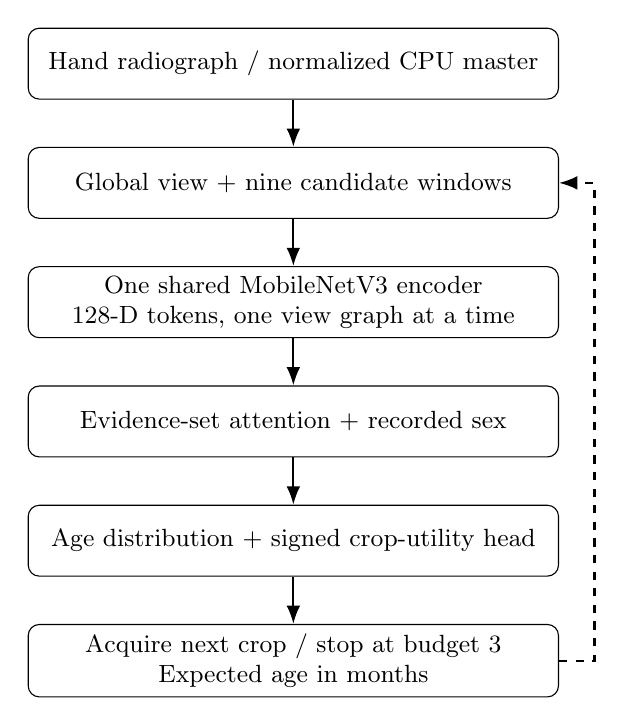
\begin{tikzpicture}[node distance=6mm,box/.style={draw,rounded corners,align=center,text width=65mm,minimum height=9mm,font=\small},arr/.style={-{Latex},thick}]
\node[box](a){Hand radiograph / normalized CPU master};
\node[box,below=of a](b){Global view + nine candidate windows};
\node[box,below=of b](c){One shared MobileNetV3 encoder\\128-D tokens, one view graph at a time};
\node[box,below=of c](d){Evidence-set attention + recorded sex};
\node[box,below=of d](e){Age distribution + signed crop-utility head};
\node[box,below=of e](f){Acquire next crop / stop at budget 3\\Expected age in months};
\draw[arr](a)--(b);\draw[arr](b)--(c);\draw[arr](c)--(d);\draw[arr](d)--(e);\draw[arr](e)--(f);
\draw[arr,dashed](f.east)--++(.45,0)|-(b.east);
\end{tikzpicture}
\caption{Implemented BARE architecture. Training enumerates all ten views with replay; deployment encodes only the global image and acquired regions.}\label{fig:architecture}\end{figure}

\subsection{Age and acquisition losses}
A normalized Gaussian target $q_m(y)\propto\exp[-(m-y)^2/8]$ supplies soft labels with a two-month width. The objective combines absolute age error, cross entropy and ordinal CDF distance:
\begin{equation}
\begin{split}
\mathcal L_{\rm age}(S,y)&=|\hat y_S-y|/12
-0.1\sum_m q_m(y)\log p_{S,m}\\
&\quad+\frac{0.5}{240}\sum_{m=0}^{239}|F_{p_S}(m)-F_q(m)|.
\end{split}
\end{equation}
Average this loss over the global-only subset, all ten views and two random subsets containing one to three local views. A 0.1-weighted mean singleton-view loss provides weak regional supervision. Background crops may receive noisy age supervision; a retrained weight ablation remains future work.

For fitting image $i$, subset $S$ and unacquired crop $j$, define the signed gain
\begin{equation}
u^*_{i,j\mid S}=|\hat y_{i,S}-y_i|-|\hat y_{i,S\cup\{j\}}-y_i|.
\end{equation}
Negative gains are retained. These are model-defined counterfactual comparisons rather than causal effects. A two-hidden-layer utility MLP predicts this gain from detached fused representation, age distribution, sex embedding, subset size, candidate geometry, normalized regional disagreement and entropy, and three cheap low-resolution statistics (mean, standard deviation, gradient energy). No unseen high-resolution token enters the utility input. The fitting-only utility objective is Huber loss with a two-month transition. Input means and scales are estimated from fitting-only utility data.

\subsection{Replay and numerical correctness}
Graph-free encoder passes first cache token values. Detached token leaves then allow differentiation of the complete fusion objective. With $g_j=\partial\mathcal L/\partial z_j$ cached, one view is replayed at a time:
\begin{equation}
\nabla_\theta\mathcal L
=\sum_j J_\theta(z_j)^\top g_j
=\nabla_\theta\sum_j\langle z_j,\sg(g_j)\rangle.
\end{equation}
Weights, augmented inputs and normalization states remain fixed until the complete optimizer update. Encoder stochastic layers are absent and running BN statistics are frozen. Fusion dropout is sampled once in the token-leaf pass; the encoder replay uses the resulting cached gradients. Under mixed precision, token gradients already include the gradient-scaler factor and are not scaled twice.

\begin{algorithm}[!t]\caption{One multiview replay update}\label{alg:replay}
\begin{algorithmic}[1]
\State Sample and retain a single master augmentation
\For{each global/local view $j$}
\State Cache $z_j=f_\theta(x_j)$ without an encoder graph
\EndFor
\State Create gradient-enabled token leaves; compute subset losses
\State Differentiate fusion once; cache scaled token gradients $g_j$
\For{each view $j$}
\State Recompute the same $z_j$ with encoder graph
\State Backpropagate $\langle z_j,\sg(g_j)\rangle$ and release graph
\EndFor
\State After the accumulation window: unscale, clip, step once
\end{algorithmic}\end{algorithm}

\subsection{Training, calibration and final inference}
The current global warmup uses seed 42; the implemented subsequent multiview stage is configured as follows. The overall run uses seed 42, AdamW weight decay $10^{-4}$, eight-image global batches, two-image multiview batches with four-step accumulation, FP16 encoder autocast, FP32 fusion/losses, and a cosine learning-rate schedule. Global encoder/head learning rates start at $10^{-4}/3\times10^{-4}$; multiview rates start at $5\times10^{-5}/1.5\times10^{-4}$. Mild brightness/contrast jitter and $\pm10^\circ$ rotations are applied coherently to the master image. There is no scale augmentation in this implementation. Global warmup is followed by multiview training, with an overnight wall-time allowance and development-based checkpoint selection. Training is in progress; completed epoch counts and checkpoint selection are pending.

Unlike the initial concept's more ambitious schedule, the implemented downstream procedure will use one fitting-only deterministic token cache per selected checkpoint and random subsets to fit the policy; augmented utility caches and trajectory-refinement cycles are not implemented. This difference is documented rather than implied to have been tested. A no-disagreement policy is implemented for subsequent fitting on the same utility targets, with that feature masked; it is not yet evaluated in these interim results.

Starting with the global token, select the unobserved crop with greatest predicted signed gain, encode it, update the evidence state and repeat up to three times. For adaptive inference, stop when the greatest gain is no larger than $\tau$. The calibration partition chooses among always-acquire, 0, 0.25, 0.5 and 1.0 months, minimizing crop count within 0.15 months MAE of the always-three policy. Model selection, fitting normalization and threshold selection precede all final holdout predictions.


\section{Results: preliminary executed experiments}
\subsection{Scope, checkpoint and dataset accounting}
This results section reports an actual frozen global-warmup checkpoint, not the completed multiview acquisition model. The snapshot is from global epoch 5 and predicts only from the whole-hand image plus recorded sex. It was chosen using development MAE during continuing training. The 1259 development images therefore serve both selection and descriptive evaluation; the resulting metrics are optimistic and must not be interpreted as independent test accuracy. No calibration or official-validation holdout predictions are used here. Table~\ref{tab:prelim_partitions} and Fig.~\ref{fig:prelim_data} document the audited dataset. Nineteen training rows with matching low-resolution hashes across the sealed holdout were conservatively excluded; no exact cross-holdout decoded-pixel duplicates were found.
\begin{table}[!t]
\centering\footnotesize
\caption{Audited partitions. Only development predictions are used in this interim results section; the final holdout remains unevaluated.}
\label{tab:prelim_partitions}
\begin{tabularx}{\columnwidth}{@{}p{27mm}XXXX@{}}
\toprule
Partition & $N$ & Female & Male & Age (mo) \\
\midrule
fit & 10077 & 4631 & 5446 & 1--228 \\
dev & 1259 & 576 & 683 & 4--228 \\
calibration & 1256 & 562 & 694 & 10--228 \\
holdout & 1425 & 652 & 773 & 3--228 \\
excluded & 19 & 9 & 10 & 48--192 \\
\bottomrule
\end{tabularx}
\end{table}
\begin{figure}[!t]
\centering
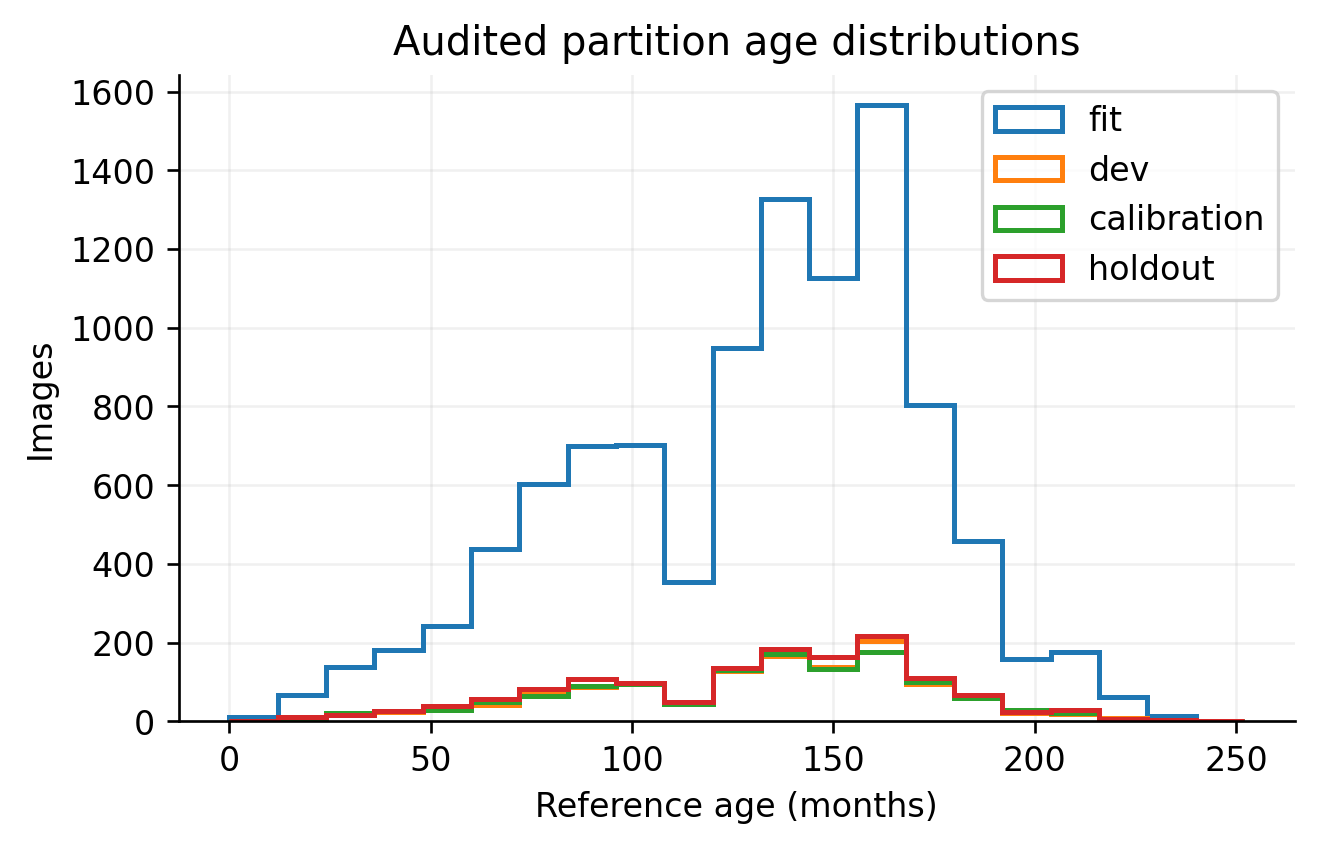
\includegraphics[width=\columnwidth]{figures/prelim_data.png}
\caption{Age distributions from the audited manifest. Holdout labels are shown for dataset accounting only; holdout images are not predicted in this interim study.}
\label{fig:prelim_data}
\end{figure}

\subsection{Prediction metrics and optimization}
The early global checkpoint obtained MAE 8.285 months and RMSE 10.928 months, with signed bias 4.496 months. Table~\ref{tab:prelim_metrics} compares its predictions against age priors whose medians are estimated from fitting labels only. The sex-specific prior selects the fitting median for the recorded sex and uses no image evidence. These priors are regression baselines rather than published deep-learning competitors. Figures~\ref{fig:prelim_scatter} and \ref{fig:prelim_agreement} show actual development predictions and errors. The agreement limits are descriptive, not clinical acceptance bounds.
\begin{table*}[!t]
\centering\footnotesize
\caption{Development-only results for a frozen global warmup checkpoint from epoch 5. This checkpoint was selected on development MAE, so these are optimistic model-selection results, not final held-out performance.}
\label{tab:prelim_metrics}
\begin{tabularx}{\textwidth}{@{}p{31mm}XXXXX@{}}
\toprule
Method & MAE & RMSE & Bias & $\leq6$ mo (\%) & $\leq12$ mo (\%) \\
\midrule
Early global checkpoint & 8.285 & 10.928 & 4.496 & 47.74 & 75.30 \\
Fitting median & 32.005 & 40.143 & 3.554 & 14.61 & 28.67 \\
Fitting sex median & 30.542 & 40.245 & 7.828 & 17.55 & 31.77 \\
\bottomrule
\end{tabularx}
\end{table*}
\begin{figure}[!t]
\centering
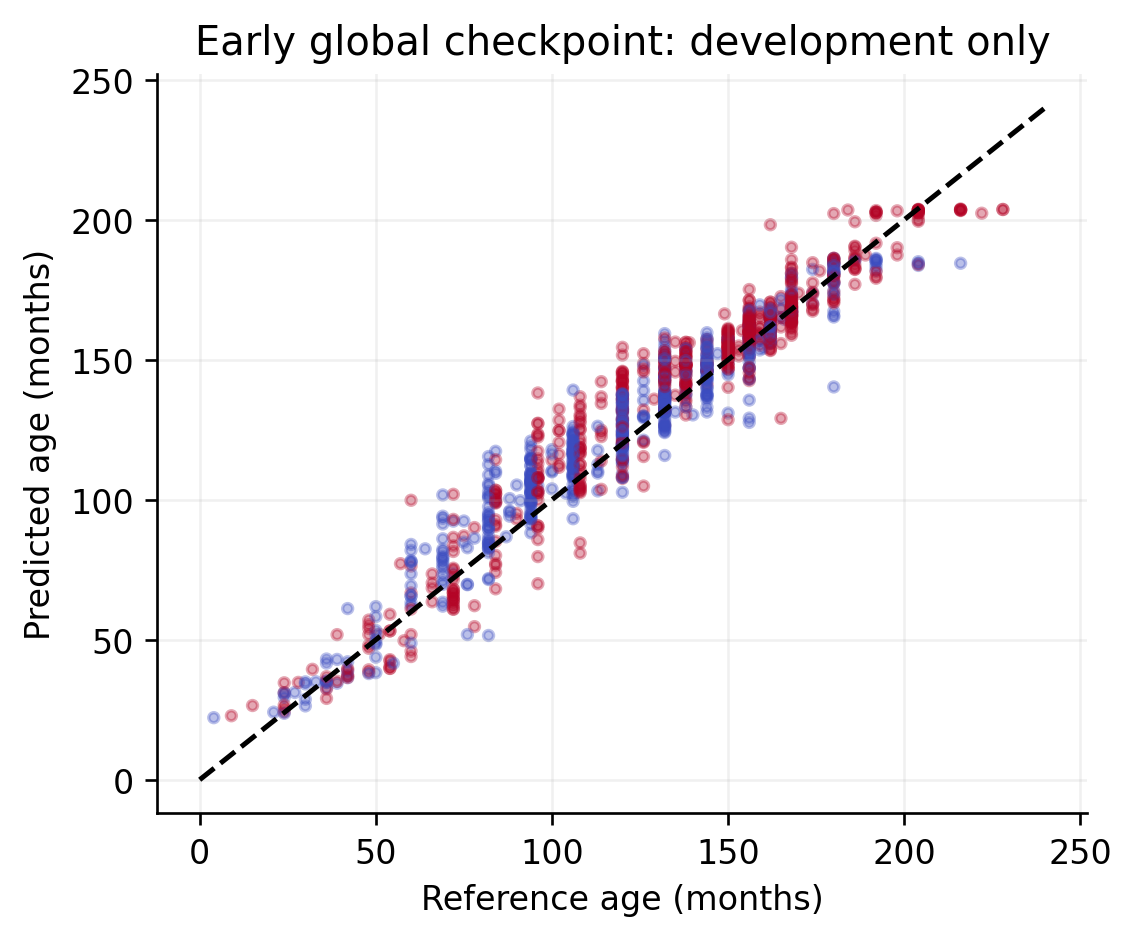
\includegraphics[width=\columnwidth]{figures/prelim_scatter.png}
\caption{Actual predictions of the frozen global warmup checkpoint on development images, colored by recorded sex.}
\label{fig:prelim_scatter}
\end{figure}
\begin{figure*}[!t]
\centering
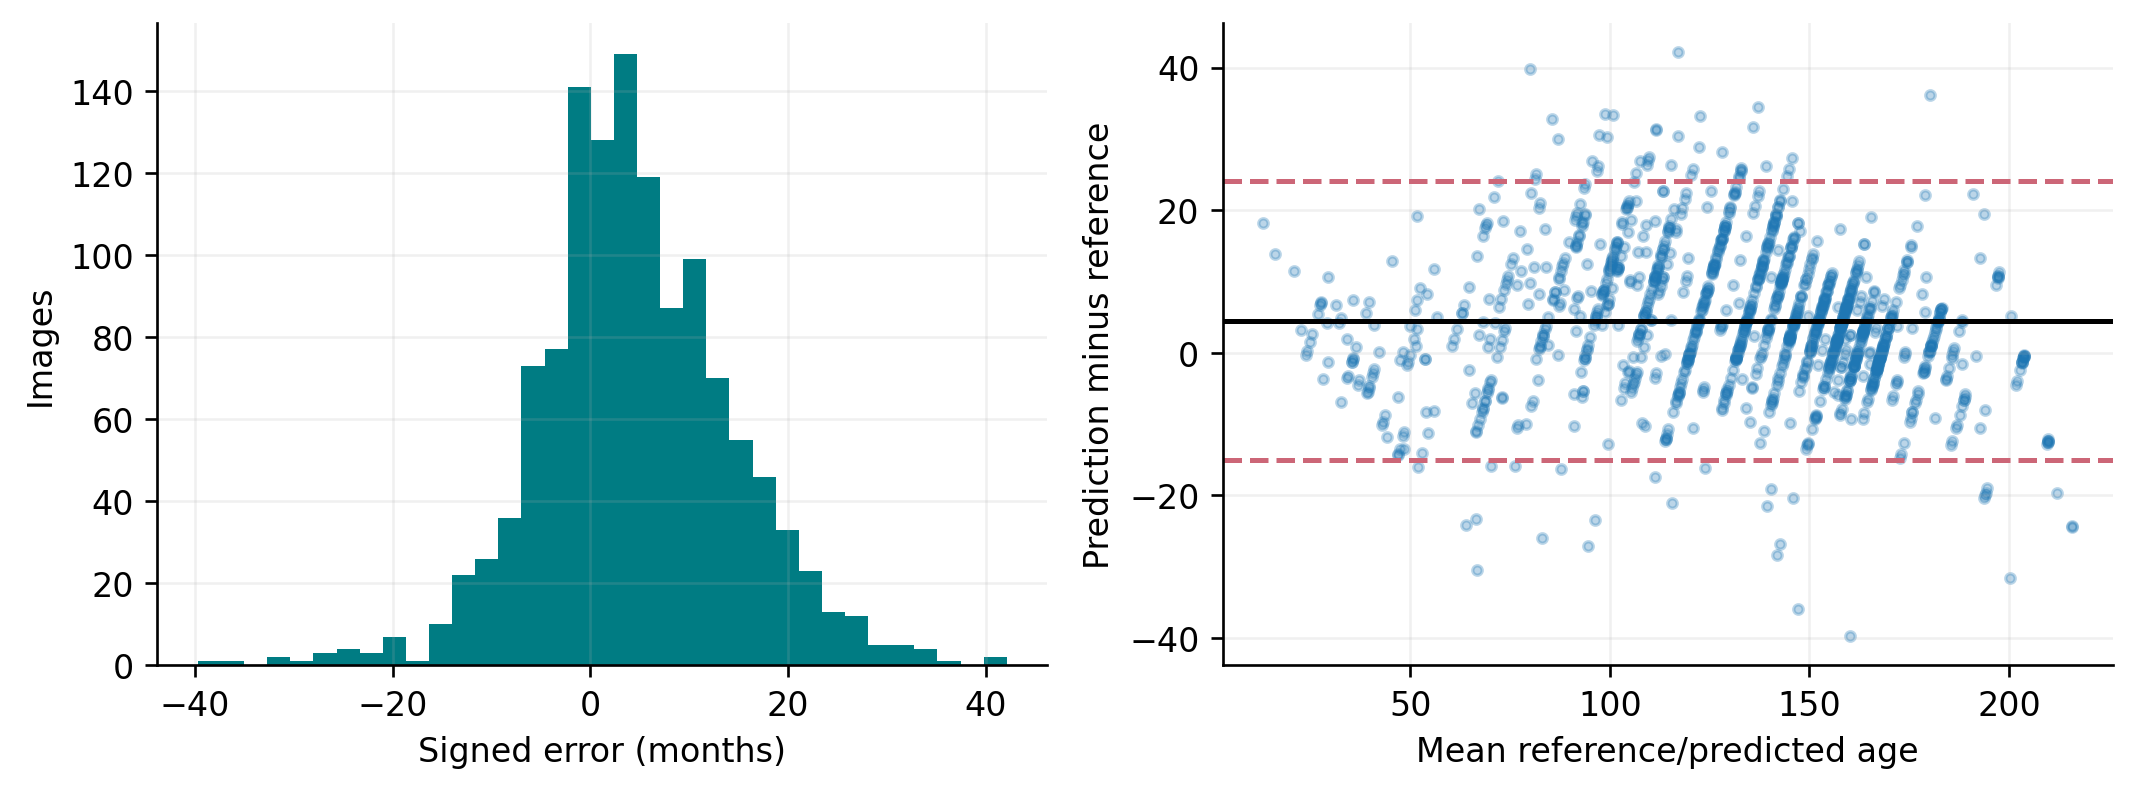
\includegraphics[width=\textwidth]{figures/prelim_agreement.png}
\caption{Development signed-error distribution and prediction--reference agreement; dashed limits are mean $\pm1.96$ standard deviations, not clinical acceptance bounds.}
\label{fig:prelim_agreement}
\end{figure*}
Figure~\ref{fig:prelim_learning} and Table~\ref{tab:prelim_epochs} show completed global optimization epochs at capture time. A temporary status-logging error occurred after the first epoch checkpoint was saved; it was repaired, and the process resumed from that checkpoint. No final holdout was evaluated during that repair. Current training is ongoing; later checkpoints and the utility policy are outside this snapshot's reported scope.
\begin{table}[!t]
\centering\footnotesize
\caption{Completed global-training epochs at capture time. Training objectives, checkpoint development MAE and training duration are actual logged values; multiview training is not yet reported here.}
\label{tab:prelim_epochs}
\begin{tabularx}{\columnwidth}{@{}p{27mm}XXXX@{}}
\toprule
Epoch & Train loss & Dev MAE & Seconds & Reserved MiB \\
\midrule
1 & 1.697 & 8.818 & 335.0 & 822.0 \\
2 & 1.215 & 9.154 & 330.4 & 834.0 \\
3 & 1.125 & 8.909 & 289.2 & 834.0 \\
4 & 1.060 & 8.404 & 263.6 & 834.0 \\
5 & 1.012 & 8.285 & 285.3 & 834.0 \\
\bottomrule
\end{tabularx}
\end{table}
\begin{figure*}[!t]
\centering
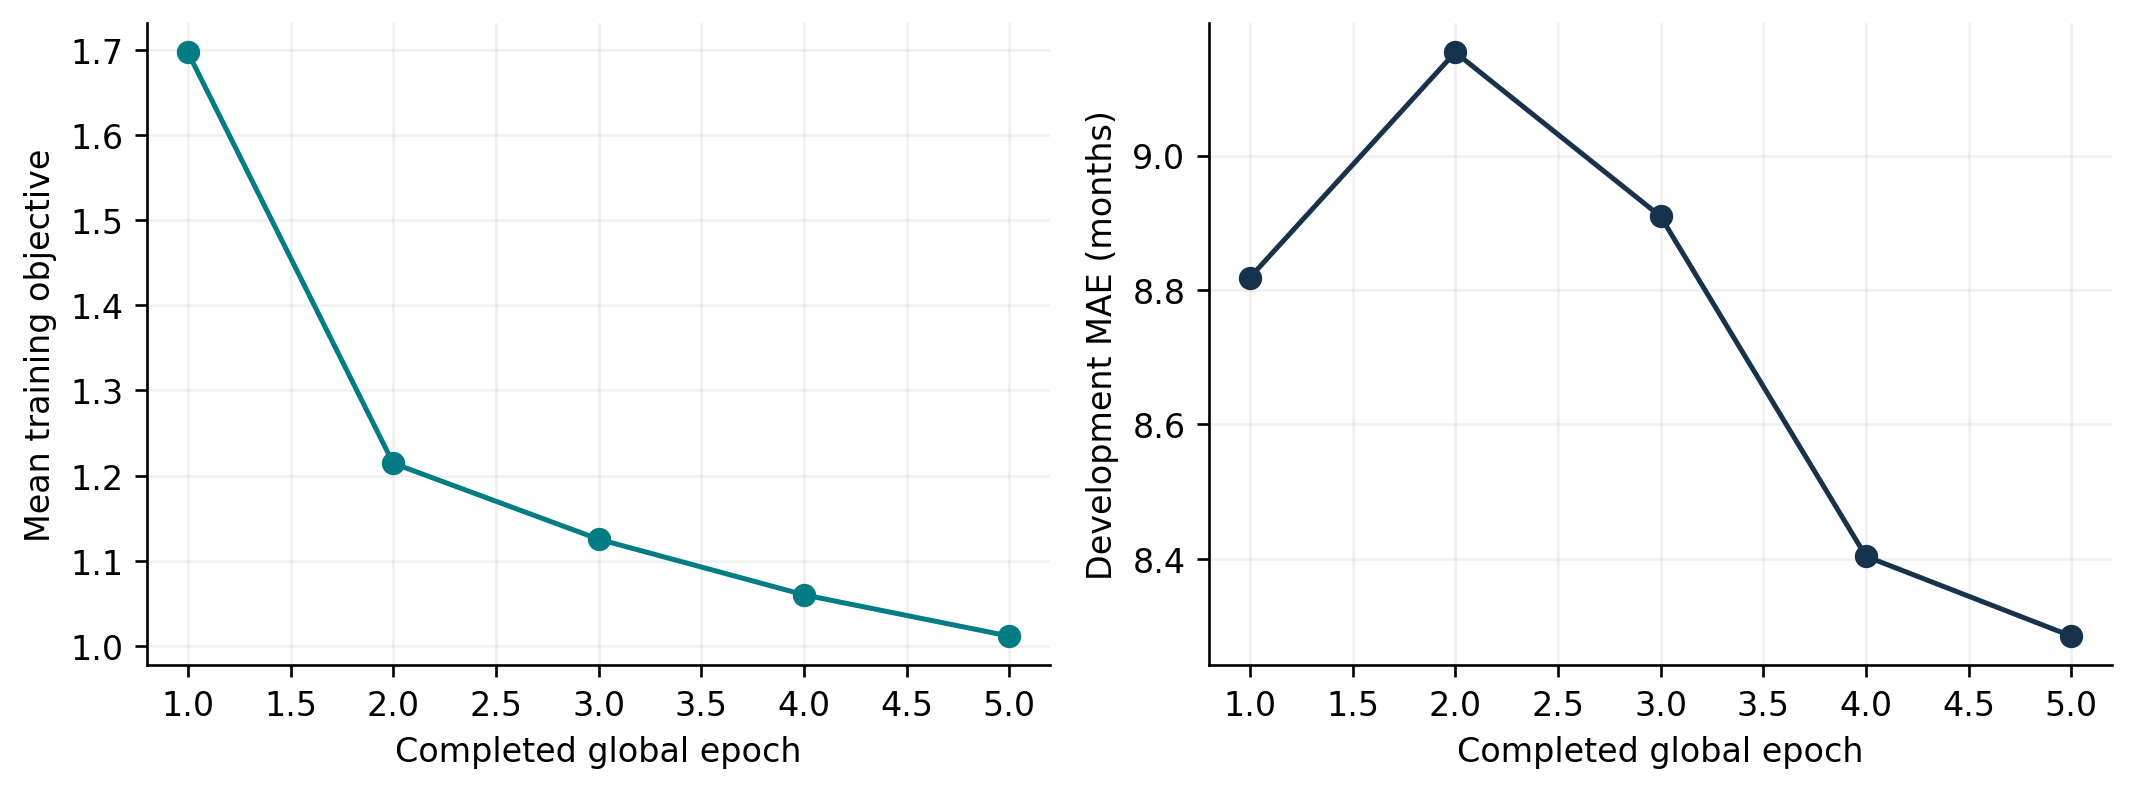
\includegraphics[width=\textwidth]{figures/prelim_learning.png}
\caption{Completed global warmup losses and development MAE at capture time. Full multiview acquisition training is not represented.}
\label{fig:prelim_learning}
\end{figure*}

\subsection{Subgroups and sampling diagnostics}
Tables~\ref{tab:prelim_sex} and \ref{tab:prelim_age} report recorded-sex and age-band metrics for the same development predictions. Figure~\ref{fig:prelim_subgroups} shows age-dependent errors and empirical absolute-error cumulative distributions, with the latter displayed up to 60 months. Small age groups and development-set selection limit interpretation. Table~\ref{tab:prelim_bootstrap} gives paired case-bootstrap differences against fitting-only median priors. The intervals condition on this single checkpoint and selected development set, so they do not estimate independent generalization or training-seed variability.
\begin{table}[!t]
\centering\footnotesize
\caption{Development recorded-sex subgroups for the same early global checkpoint.}
\label{tab:prelim_sex}
\begin{tabularx}{\columnwidth}{@{}p{27mm}XXXX@{}}
\toprule
Group & $N$ & MAE & RMSE & Bias \\
\midrule
Female & 576 & 8.162 & 10.727 & 4.528 \\
Male & 683 & 8.389 & 11.094 & 4.470 \\
\bottomrule
\end{tabularx}
\end{table}
\begin{table}[!t]
\centering\footnotesize
\caption{Development age-band results in months; small subgroups should be interpreted cautiously.}
\label{tab:prelim_age}
\begin{tabularx}{\columnwidth}{@{}p{27mm}XXXX@{}}
\toprule
Age (mo) & $N$ & MAE & RMSE & $\leq6$ (\%) \\
\midrule
0--47 & 44 & 5.169 & 6.762 & 70.5 \\
48--95 & 228 & 11.034 & 13.559 & 28.9 \\
96--143 & 439 & 10.583 & 12.976 & 34.4 \\
144--191 & 500 & 5.187 & 7.169 & 67.2 \\
192--240 & 48 & 9.340 & 11.906 & 35.4 \\
\bottomrule
\end{tabularx}
\end{table}
\begin{table}[!t]
\centering\footnotesize
\caption{Development case-bootstrap difference in MAE (early global model minus fitting-only age prior), 2,000 replicates. Negative favors the image model. Development selection and one training seed limit inference; these are not independent test-set confidence intervals.}
\label{tab:prelim_bootstrap}
\begin{tabularx}{\columnwidth}{@{}p{27mm}XX@{}}
\toprule
Comparator & $\Delta$ MAE & 95\% interval \\
\midrule
Fitting median & -23.720 & [-25.056, -22.416] \\
Fitting sex median & -22.257 & [-23.732, -20.854] \\
\bottomrule
\end{tabularx}
\end{table}
\begin{figure*}[!t]
\centering
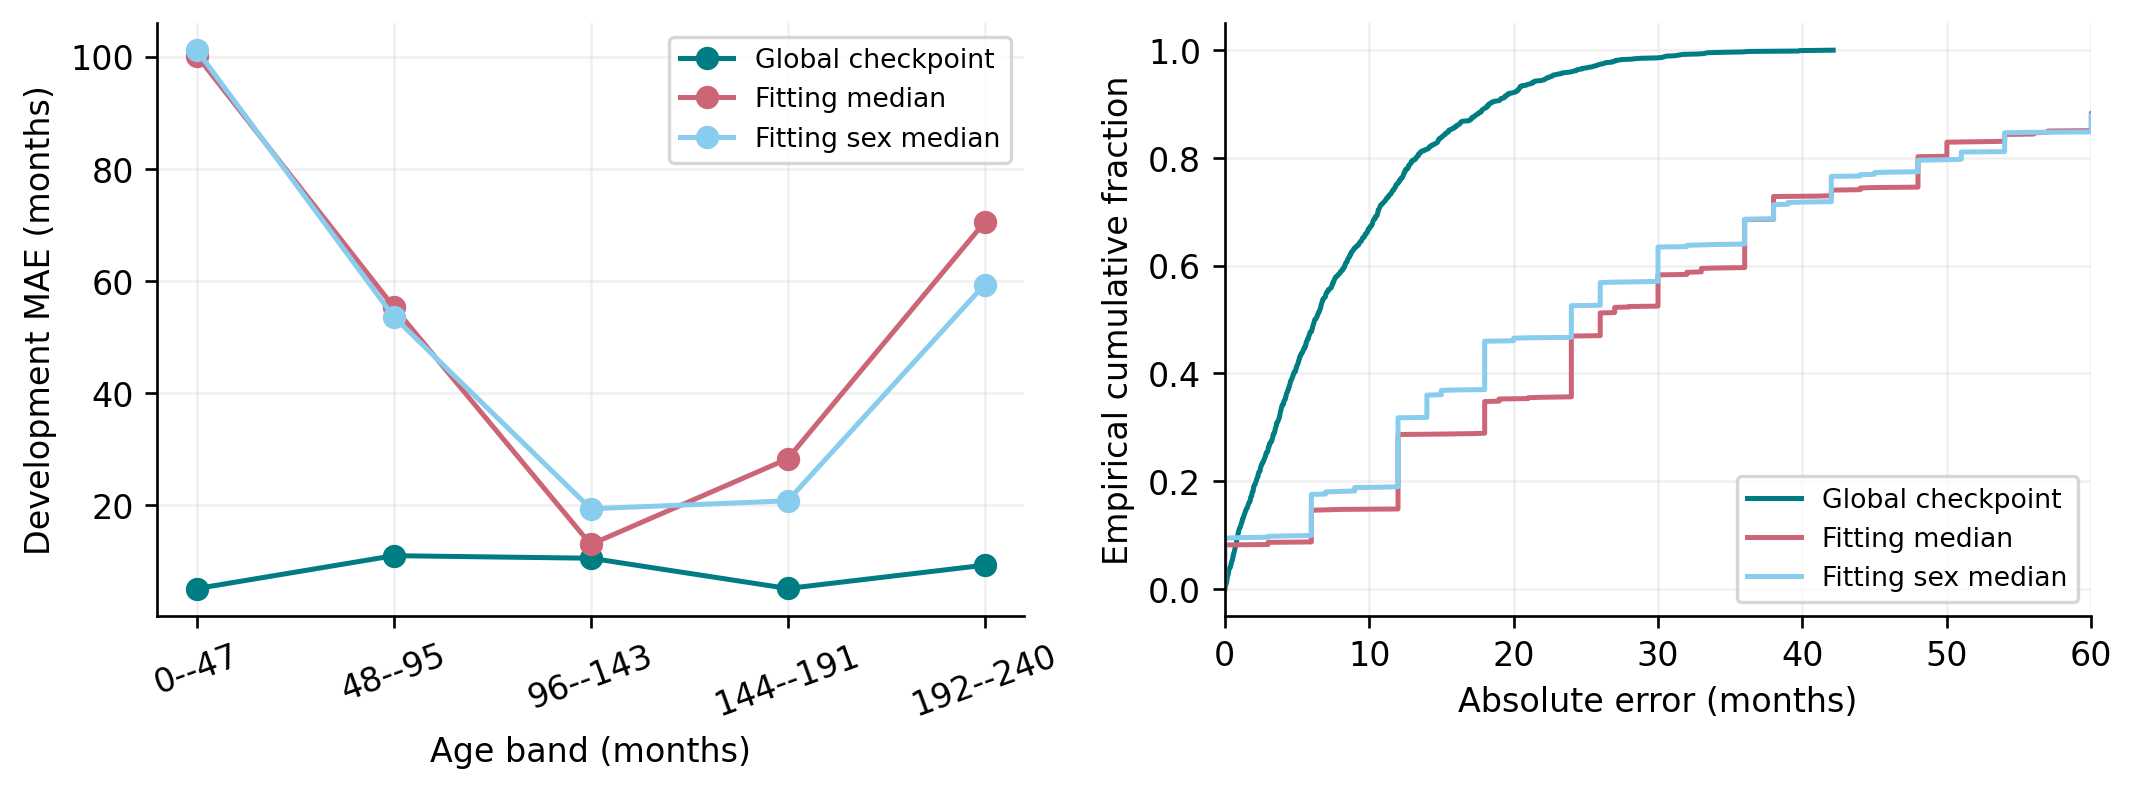
\includegraphics[width=\textwidth]{figures/prelim_subgroups.png}
\caption{Development age-band error and empirical absolute-error distributions versus fitting-only median priors.}
\label{fig:prelim_subgroups}
\end{figure*}

\subsection{GPU resources and implementation checks}
Table~\ref{tab:prelim_memory} and Fig.~\ref{fig:prelim_resources} report an executed ten-view synthetic-input training profile on the RTX 3050. Twenty-two complete optimizer updates were profiled, with the first two excluded from timing. Joint backpropagation reserved 704 MiB and replay reserved 260 MiB, but replay took more time per update. Both fitted the 4 GB device: this is a headroom/compute tradeoff rather than proof that joint training was impossible. These memory measurements are separate from the global checkpoint's accuracy experiment. CUDA allocator metrics do not include every driver allocation; sampled device use is listed separately.
\begin{table}[!t]
\centering\footnotesize
\caption{Ten-view synthetic-input admission profile on the RTX 3050, batch two; 22 complete optimizer updates per mode, first two excluded from timing. Both modes fit 4 GB. Device use is sampled, not a continuously measured peak.}
\label{tab:prelim_memory}
\begin{tabularx}{\columnwidth}{@{}p{27mm}XXXX@{}}
\toprule
Mode & Allocated MiB & Reserved MiB & Device MiB & s/update \\
\midrule
joint & 687.5 & 704.0 & 819 & 0.225 \\
replay & 192.3 & 260.0 & 375 & 0.345 \\
\bottomrule
\end{tabularx}
\end{table}
\begin{figure*}[!t]
\centering
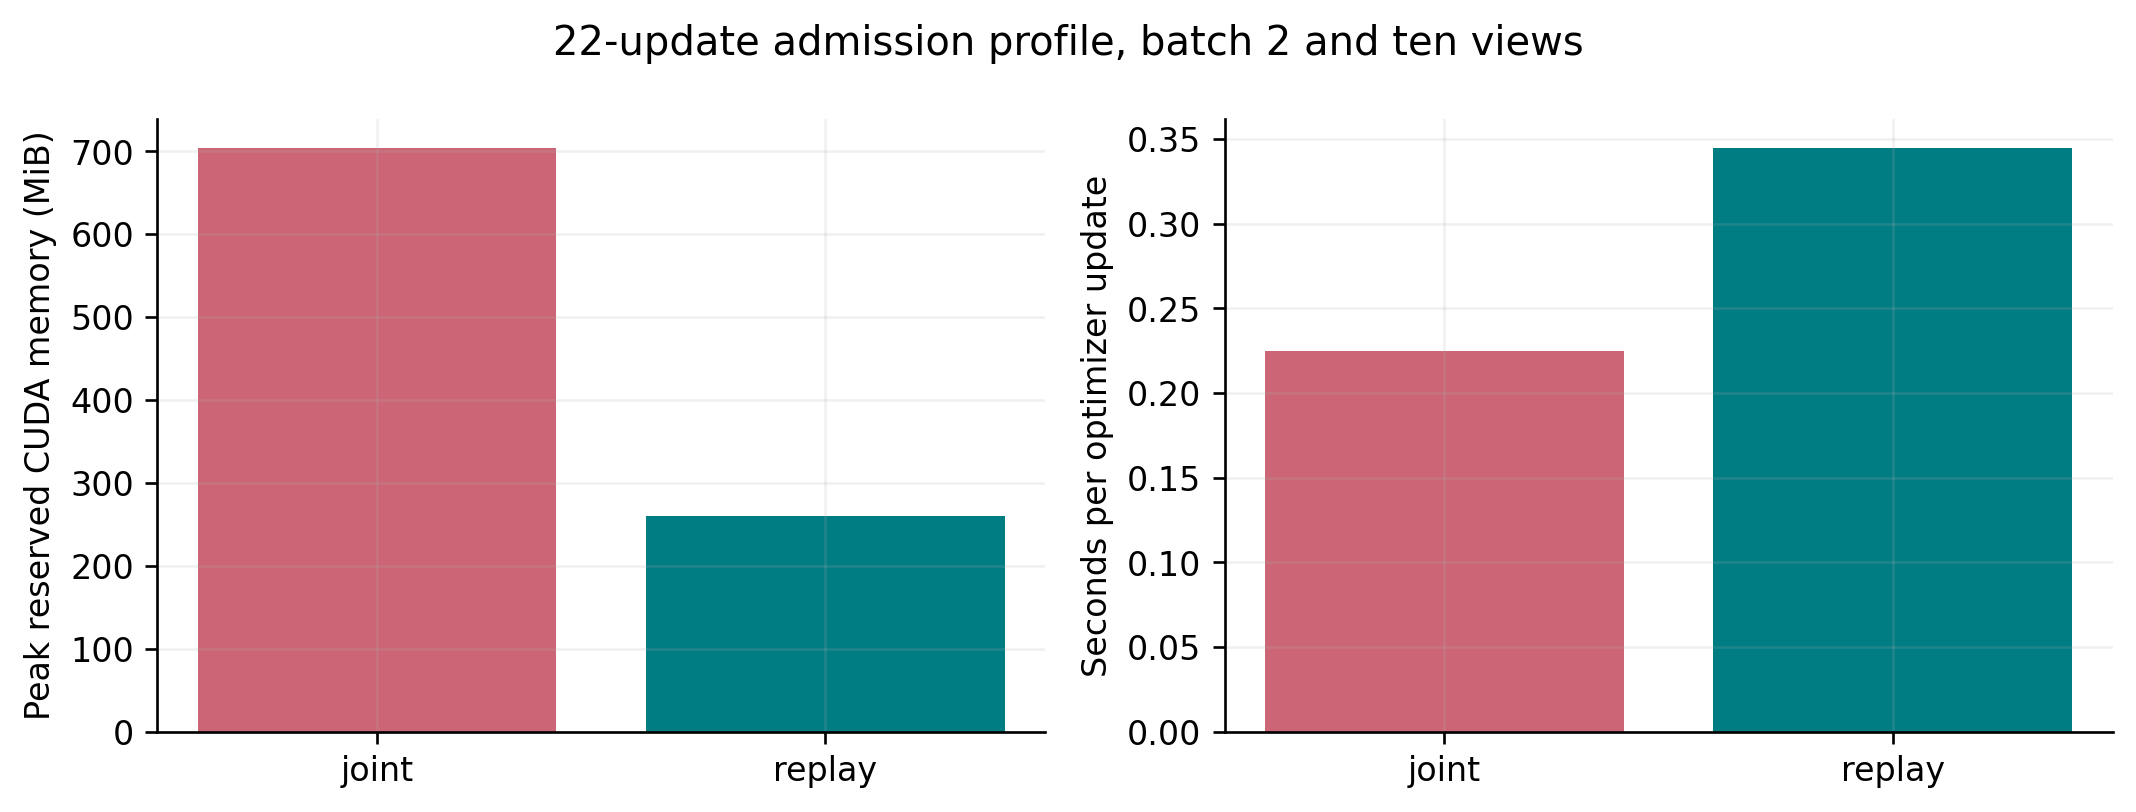
\includegraphics[width=\textwidth]{figures/prelim_resources.png}
\caption{Actual same-hardware ten-view admission measurements: replay reserves less CUDA memory while taking more time per optimizer update.}
\label{fig:prelim_resources}
\end{figure*}
The three-view deterministic FP32 replay test in Table~\ref{tab:prelim_replay} obtained relative encoder-gradient error $4.54\times10^{-8}$ and zero fusion-gradient discrepancy. It verifies the implementation on a small case, not convergence or clinical prediction quality. Table~\ref{tab:prelim_checks} lists executed acquisition-input, crop-budget, stopping and sex-parsing checks. The policy-isolation check uses test tensors rather than trained policy-accuracy results.
\begin{table}[!t]
\centering\footnotesize
\caption{Actual deterministic FP32 gradient-replay equivalence test, three views at 64-pixel resolution.}
\label{tab:prelim_replay}
\begin{tabularx}{\columnwidth}{@{}p{27mm}X@{}}
\toprule
Quantity & Value \\
\midrule
encoder max absolute error & 3.725e-09 \\
encoder relative l2 error & 4.540e-08 \\
fusion max absolute error & 0.000e+00 \\
passed & True \\
precision & FP32 \\
views & 3 \\
resolution & 64 \\
\bottomrule
\end{tabularx}
\end{table}
\begin{table}[!t]
\centering\footnotesize
\caption{Executed software checks. Unseen-isolation zero means altering unavailable encoded crops leaves policy input features exactly unchanged.}
\label{tab:prelim_checks}
\begin{tabularx}{\columnwidth}{@{}p{27mm}X@{}}
\toprule
Check & Measured outcome \\
\midrule
unseen isolation [0] & 0.0 \\
unseen isolation [0, 2] & 0.0 \\
unseen isolation [0, 2, 7] & 0.0 \\
budget 0 & True \\
budget 1 & True \\
budget 2 & True \\
budget 3 & True \\
immediate stop equals global & True \\
invalid sex rejected & True \\
\bottomrule
\end{tabularx}
\end{table}

\subsection{Five genuine development Grad-CAM images}
Figures~\ref{fig:prelim_gradcam_1}--\ref{fig:prelim_gradcam_5} contain five actual hand radiographs with regression Grad-CAM computed from the frozen trained global checkpoint. Cases are selected by the smallest image ID in each prespecified 48-month development age band, not by prediction error or attractiveness. Table~\ref{tab:prelim_cam_cases} identifies every case and distinguishes FP16 evaluation from FP32 attribution. For the predicted expected age and last convolutional maps,
\begin{equation}
\alpha_k=\frac1{HW}\sum_{u,v}\frac{\partial\hat y}{\partial A^k_{uv}},\qquad
G=\operatorname{ReLU}\left(\sum_k\alpha_kA^k\right).
\end{equation}
Each map is normalized by its positive maximum. Positive scalar-age saliency indicates features locally increasing age; negative contributions are omitted. Color values are not comparable magnitudes across cases. These are whole-hand maps from the global warmup model, not trained acquisition-policy or local-crop explanations. Saliency cannot establish causal anatomy, clinical reasoning or localization correctness.
\begin{table}[!t]
\centering\footnotesize
\caption{Five genuine Grad-CAM cases from development data. Lowest ID in each prespecified age band; no selection by low error or attractive saliency. FP32 attribution and FP16 evaluation are listed separately.}
\label{tab:prelim_cam_cases}
\begin{tabularx}{\columnwidth}{@{}p{27mm}XXXX@{}}
\toprule
ID & Age band & Target & Eval. & Attrib. \\
\midrule
1398 & 0--47 & 4 & 22.17 & 22.19 \\
1394 & 48--95 & 57 & 77.17 & 77.13 \\
1393 & 96--143 & 132 & 131.29 & 131.32 \\
1384 & 144--191 & 156 & 156.48 & 156.47 \\
1617 & 192--240 & 192 & 184.50 & 184.51 \\
\bottomrule
\end{tabularx}
\end{table}
\begin{figure*}[!t]
\centering
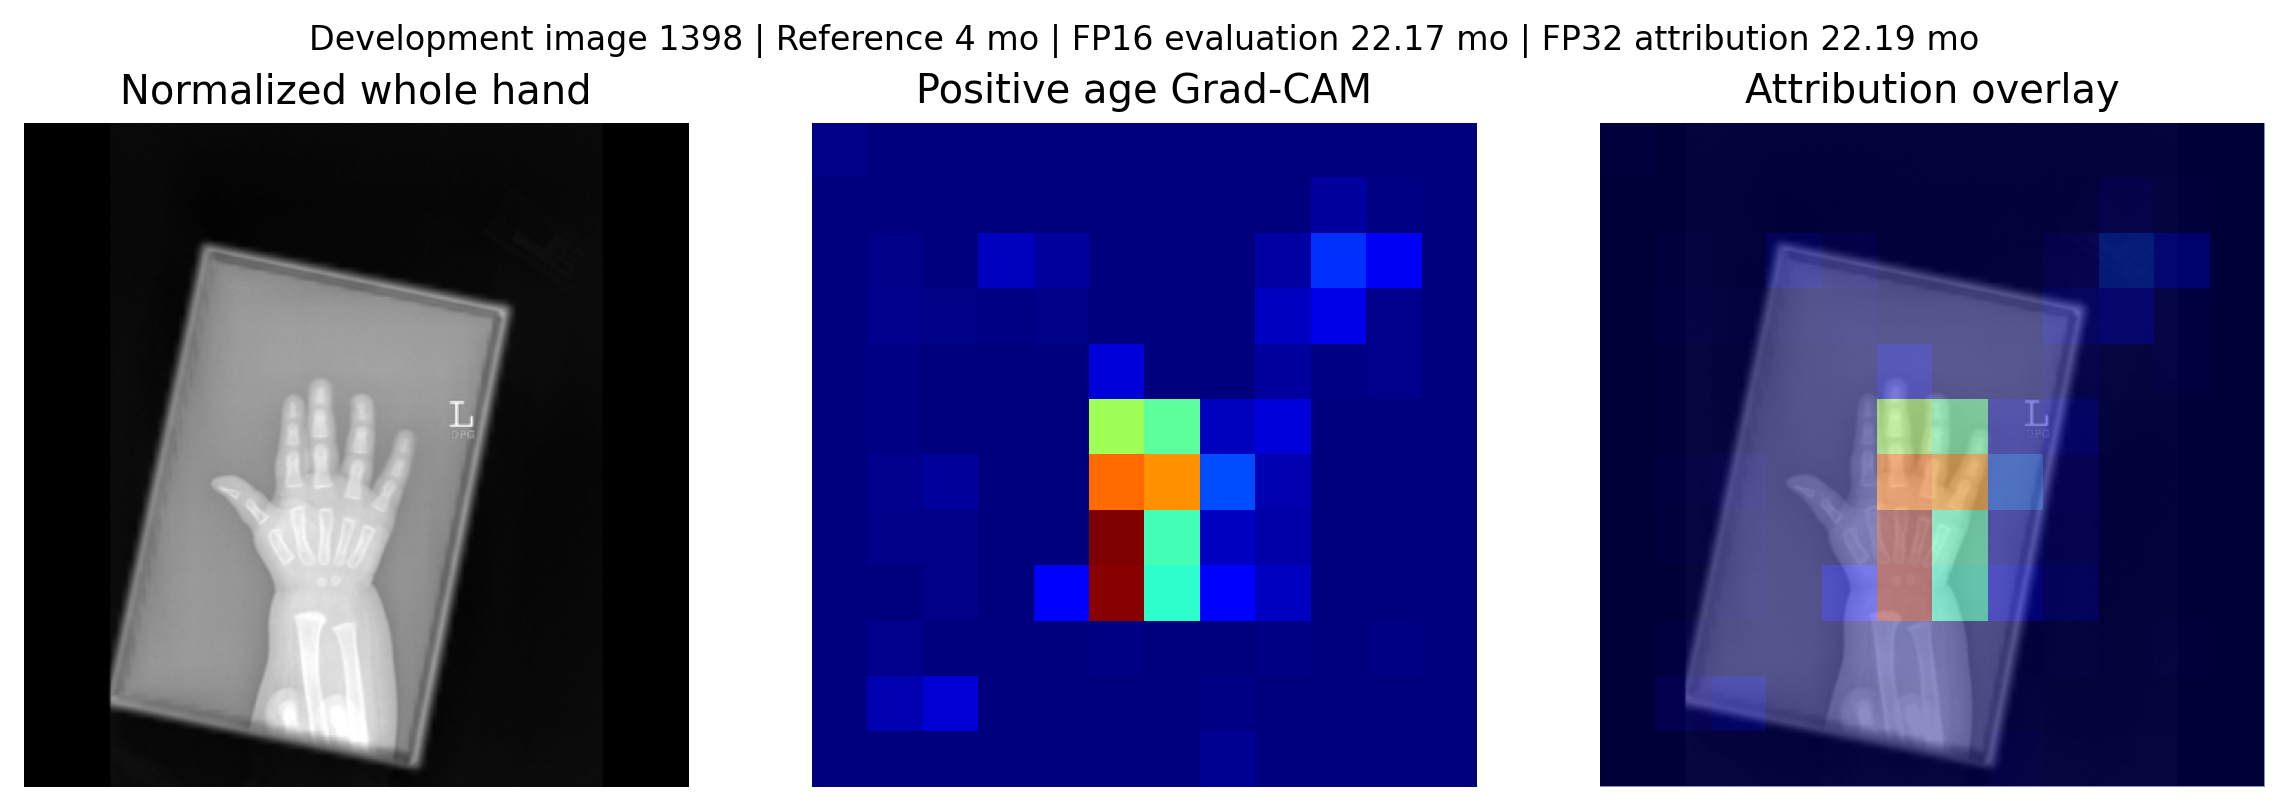
\includegraphics[width=\textwidth]{figures/prelim_gradcam_1.png}
\caption{Development Grad-CAM case 1, image 1398, reference age 4 months. Original normalized hand, positive expected-age attribution and overlay from the frozen global checkpoint. This is not a learned crop-policy explanation.}
\label{fig:prelim_gradcam_1}
\end{figure*}
\begin{figure*}[!t]
\centering
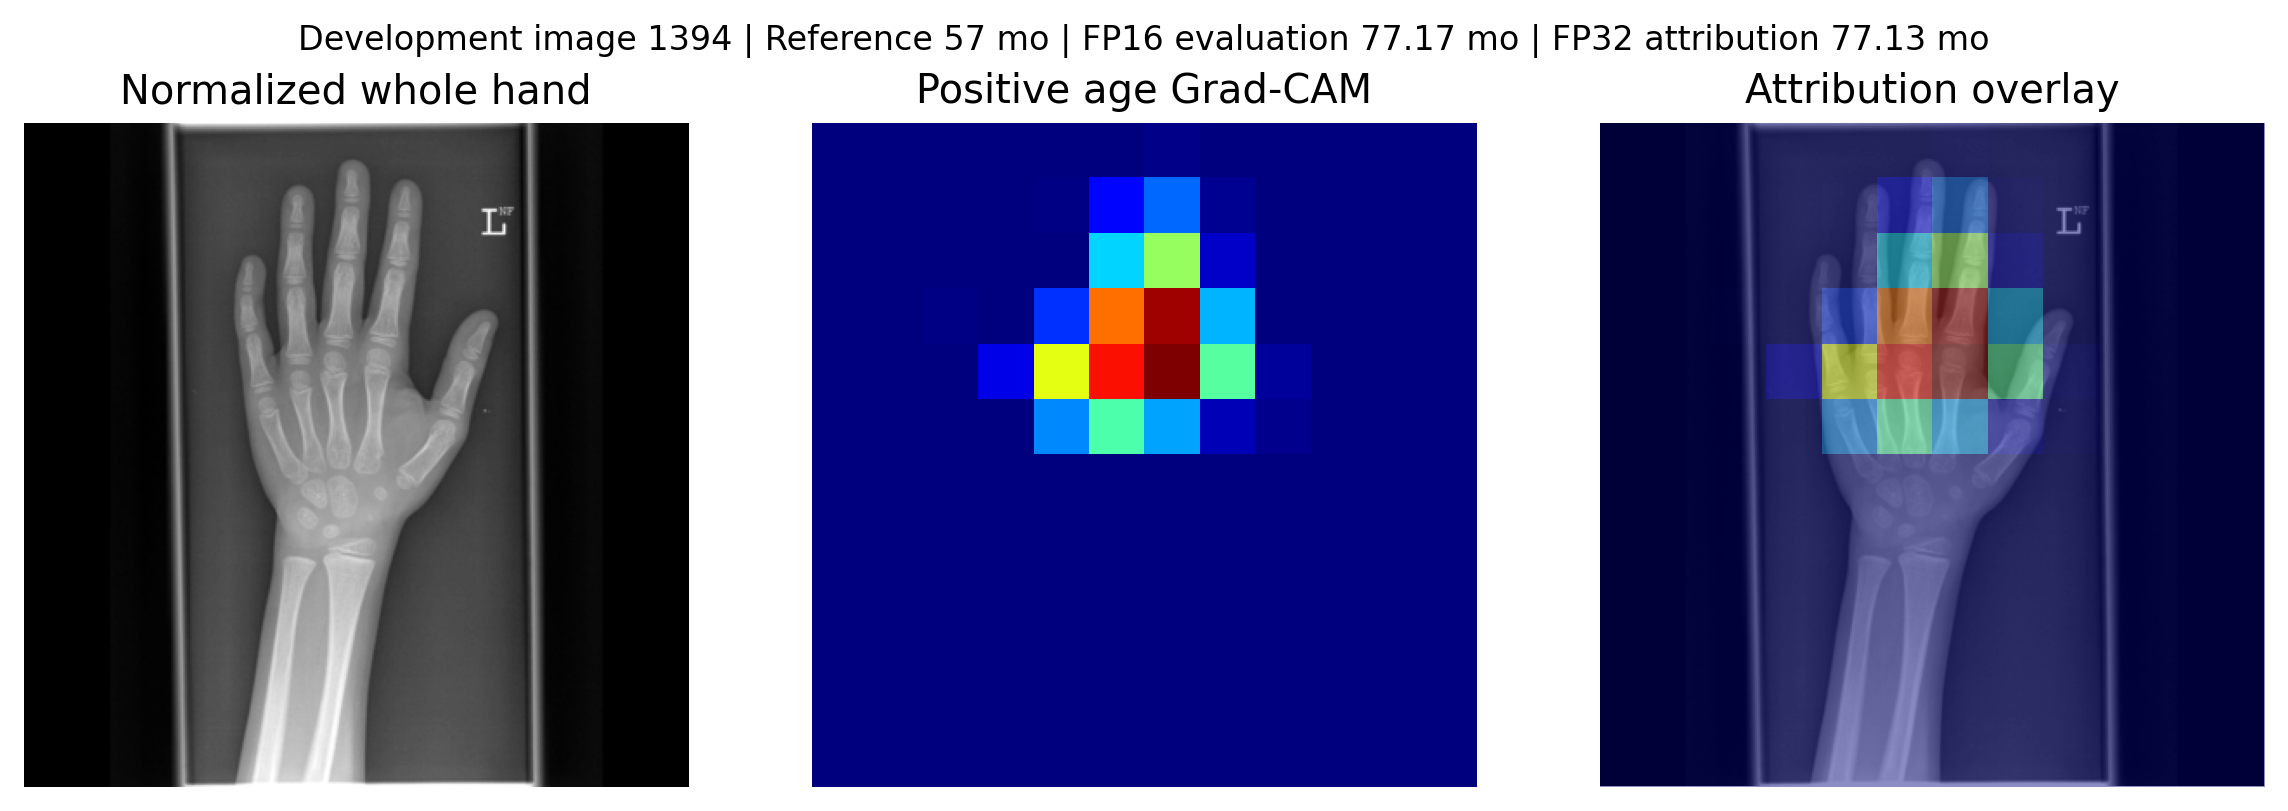
\includegraphics[width=\textwidth]{figures/prelim_gradcam_2.png}
\caption{Development Grad-CAM case 2, image 1394, reference age 57 months. Original normalized hand, positive expected-age attribution and overlay from the frozen global checkpoint. This is not a learned crop-policy explanation.}
\label{fig:prelim_gradcam_2}
\end{figure*}
\begin{figure*}[!t]
\centering
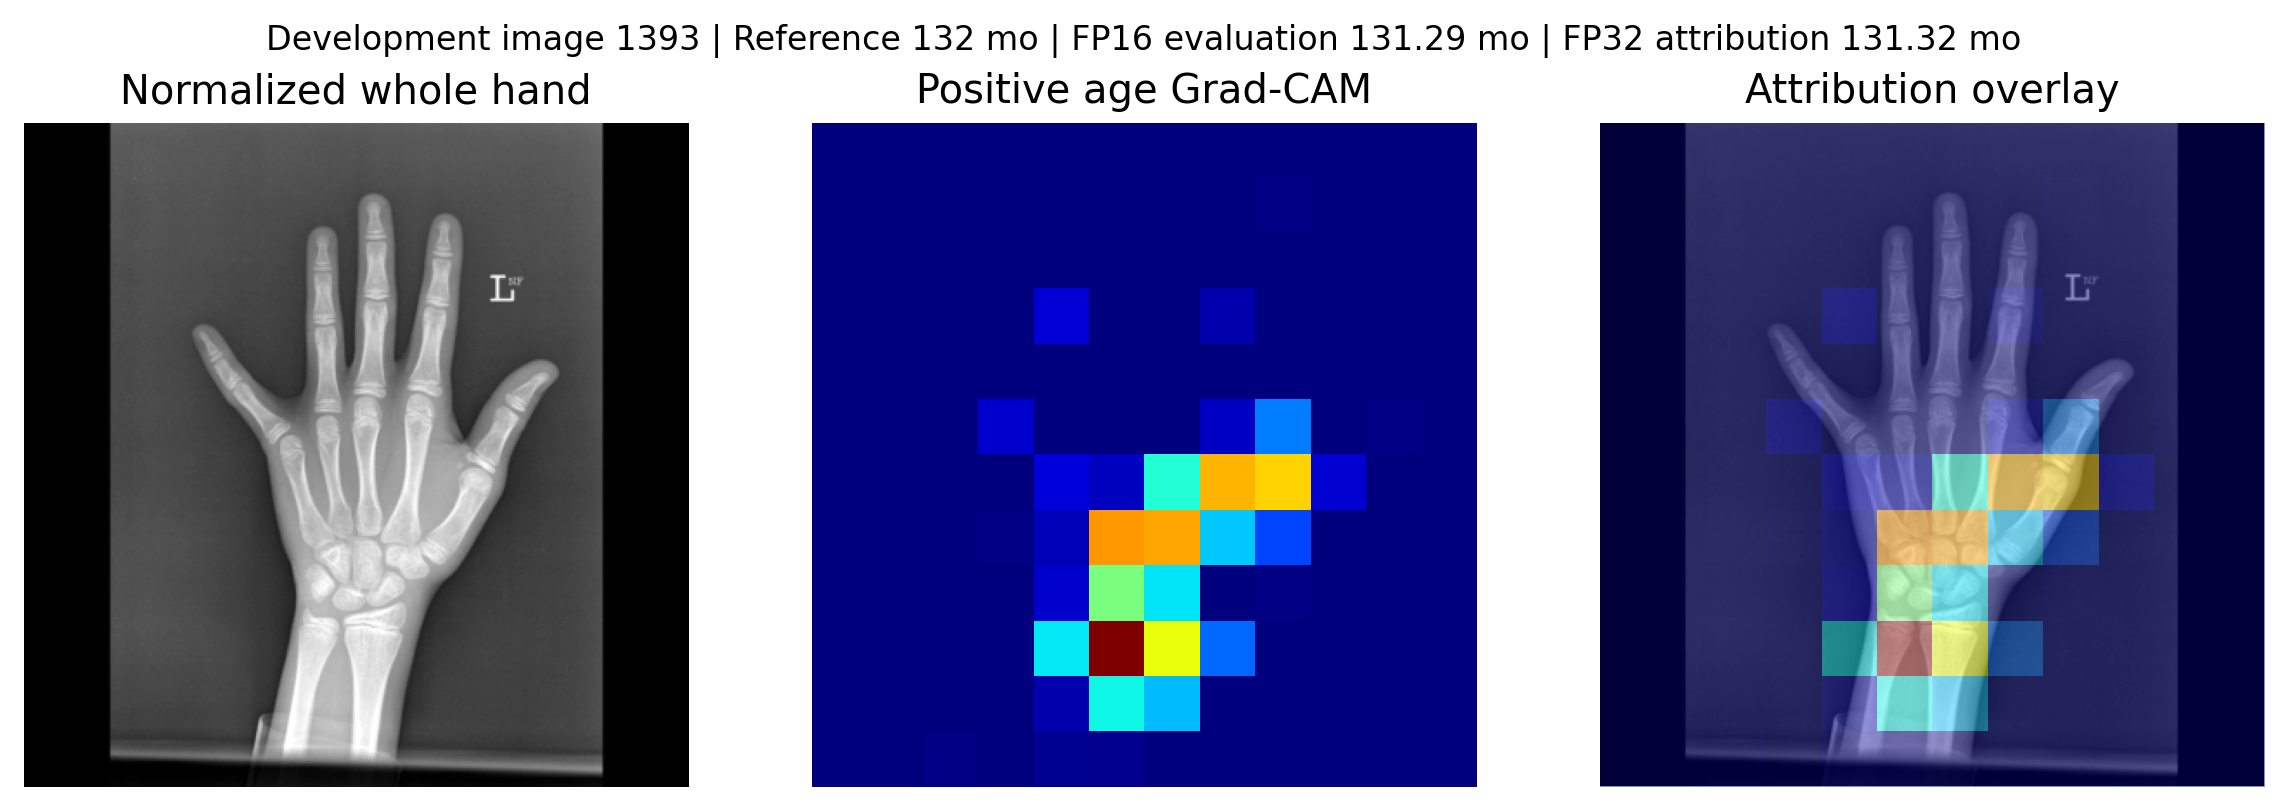
\includegraphics[width=\textwidth]{figures/prelim_gradcam_3.png}
\caption{Development Grad-CAM case 3, image 1393, reference age 132 months. Original normalized hand, positive expected-age attribution and overlay from the frozen global checkpoint. This is not a learned crop-policy explanation.}
\label{fig:prelim_gradcam_3}
\end{figure*}
\begin{figure*}[!t]
\centering
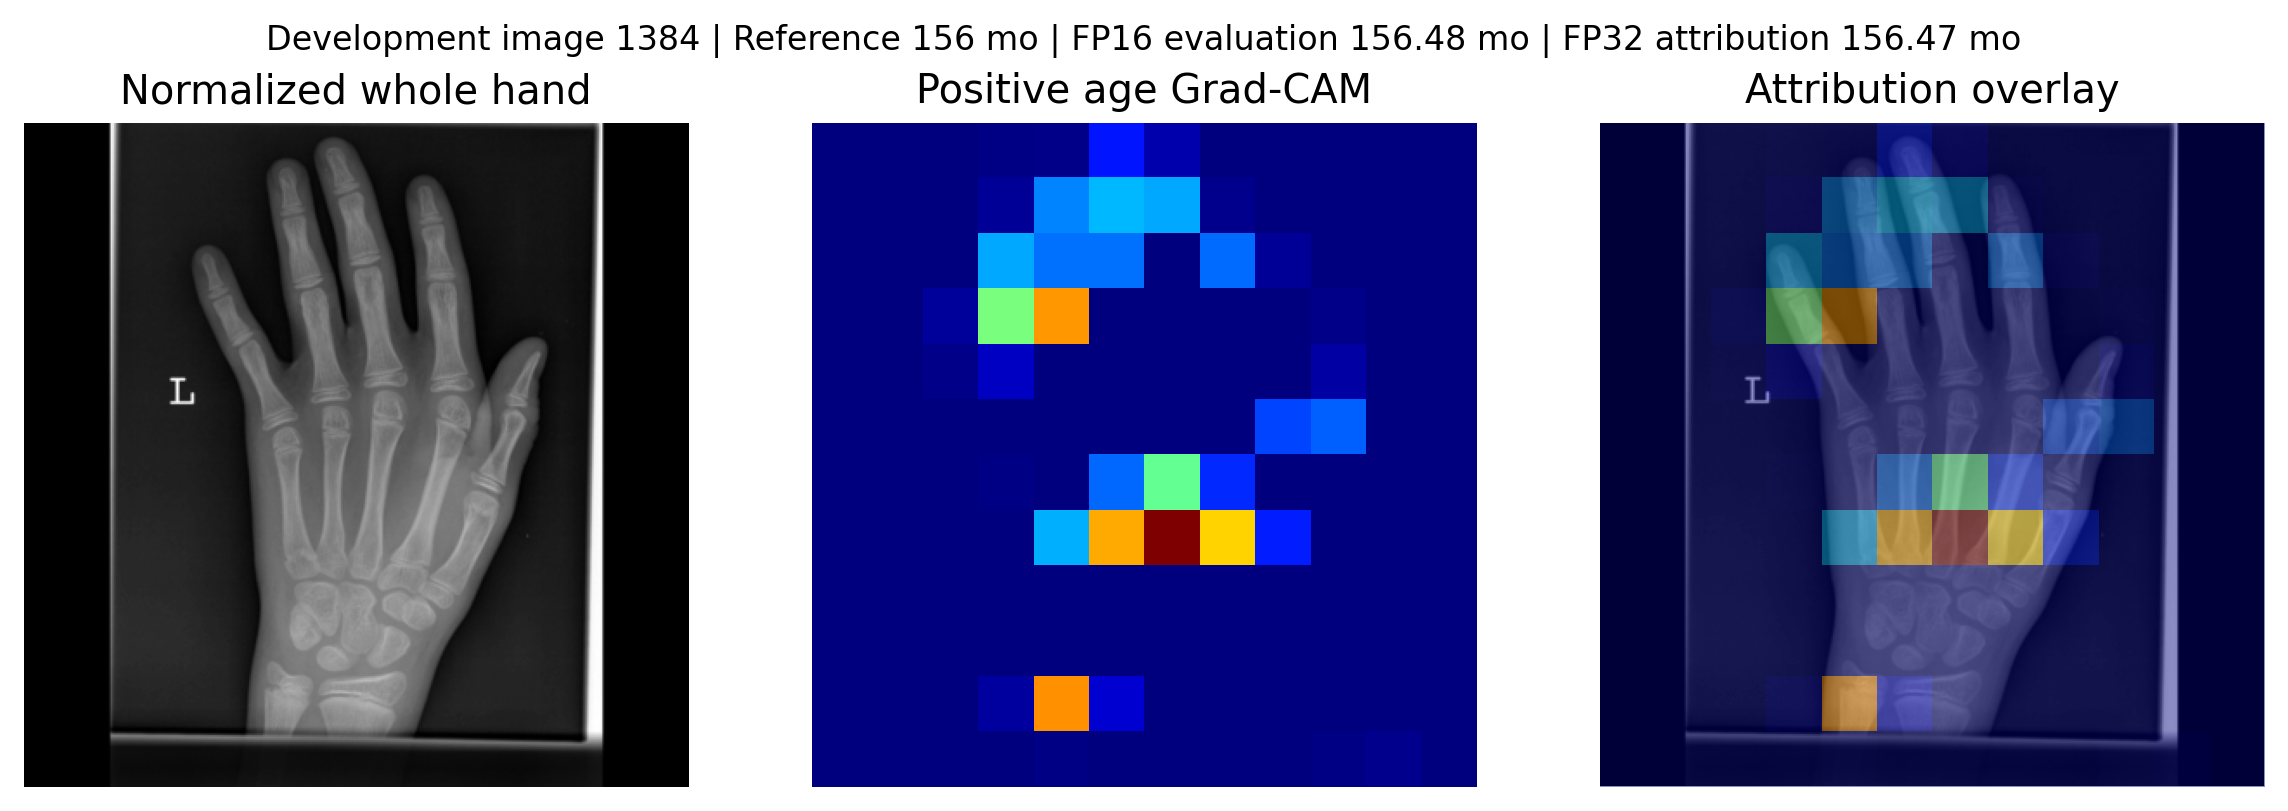
\includegraphics[width=\textwidth]{figures/prelim_gradcam_4.png}
\caption{Development Grad-CAM case 4, image 1384, reference age 156 months. Original normalized hand, positive expected-age attribution and overlay from the frozen global checkpoint. This is not a learned crop-policy explanation.}
\label{fig:prelim_gradcam_4}
\end{figure*}
\begin{figure*}[!t]
\centering
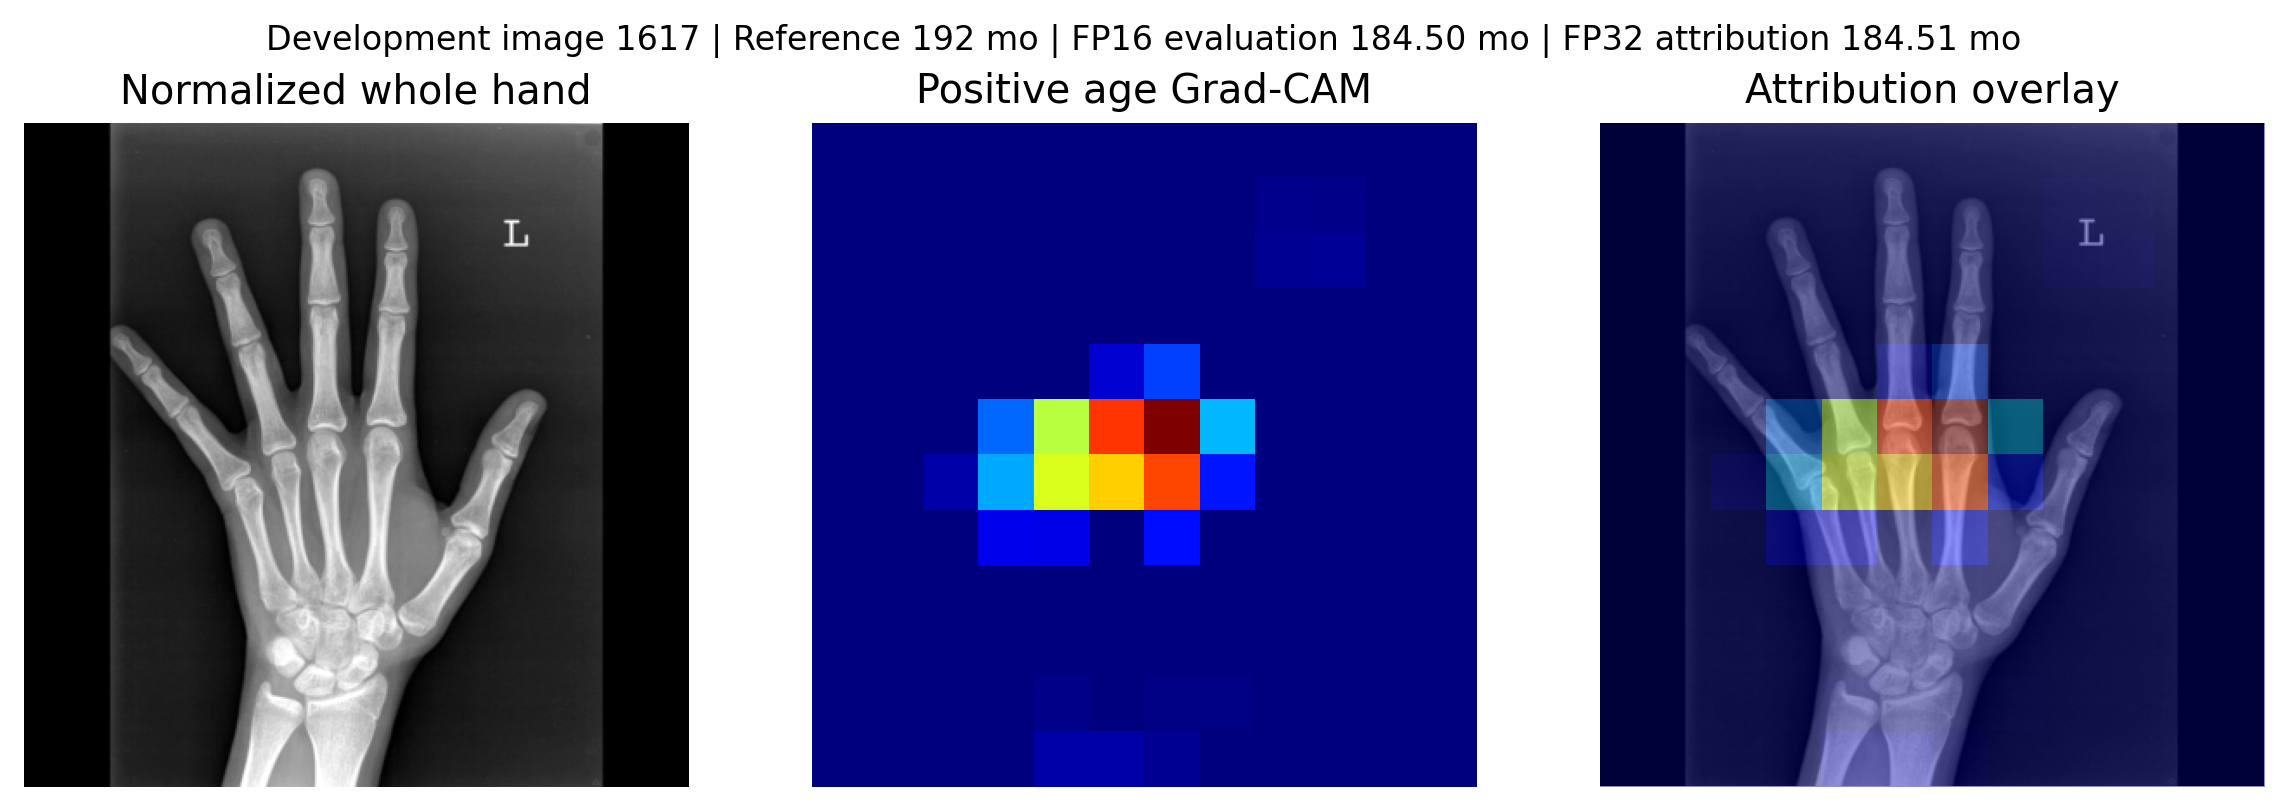
\includegraphics[width=\textwidth]{figures/prelim_gradcam_5.png}
\caption{Development Grad-CAM case 5, image 1617, reference age 192 months. Original normalized hand, positive expected-age attribution and overlay from the frozen global checkpoint. This is not a learned crop-policy explanation.}
\label{fig:prelim_gradcam_5}
\end{figure*}

\subsection{Comprehensive published-method comparison}
Tables~\ref{tab:prelim_sota_accuracy}, \ref{tab:prelim_sota_resources} and \ref{tab:prelim_sota_optimization} cover reported accuracy, evaluation protocol, architecture, supervision, resolution, GPU, batch size, epochs, parameters, FLOPs, VRAM, latency, optimizer, learning rate, objective, data sizes and training duration. NR means not verified/reported in the consulted source material; these missing values are not estimated from backbone names. Published results use different official/custom test partitions and annotations. Our early checkpoint uses development data, so no direct SOTA ranking is valid. Resource profiles and prediction metrics likewise describe separate executed experiments, and latencies measured on different GPUs are not comparable.
\begin{table*}[!t]
\centering\footnotesize
\caption{Published strong-method accuracy and supervision comparison. Published official-test results are not directly comparable to this development-only early checkpoint. RFGA RMSE uses Table 1 (4.02). NR = not verified/reported in consulted material; no SOTA claim.}
\label{tab:prelim_sota_accuracy}
\begin{tabularx}{\textwidth}{@{}p{31mm}XXXXX@{}}
\toprule
Method & MAE (mo) & RMSE (mo) & Evaluation & Backbone / fusion & Auxiliary inputs \\
\midrule
Chen et al.~\cite{chen} & 4.40 & 4.78 & Official test 200 & Attention-guided multiview & No keypoints \\
RFGA-Net~\cite{rfga} & 3.34 & 4.02 & Official test 200 & InceptionV3 + RAA/FFA & Sex; attention \\
CFJLNet~\cite{cfjl} & 4.07 & NR & Official test (as cited) & Coarse/fine attention & Attention \\
BoGFF-Net~\cite{bogff} & 3.91 & NR & Official test 200 & Multiscale self-attention & Sex; triplet objective \\
Divide/conquer~\cite{lightweight} & 3.90 & NR & RSNA test; 0--20 yr & Lightweight regional CNNs & Regional decomposition \\
BoNet+~\cite{bonetplus} & 3.81 & NR & Official test 200 & InceptionV3 + transformer & Keypoints / boxes \\
DSGTF~\cite{stage} & 4.82 & NR & Custom test 1,892 & InceptionV3 + EfficientNet-B1 & 17 keypoints \\
Early global checkpoint & 8.285 & 10.928 & Development 1,259 & MobileNetV3 + attention & Sex; no keypoints \\
\bottomrule
\end{tabularx}
\end{table*}
\begin{table*}[!t]
\centering\footnotesize
\caption{Published model/resource comparison. Values marked NR are not inferred. Warmup uses only the global image; profile-table replay memory refers to a separate ten-view experiment. VRAM here is peak allocator-reserved warmup memory. Latencies on different hardware are not comparable.}
\label{tab:prelim_sota_resources}
\begin{tabularx}{\textwidth}{@{}p{28mm}XXXXXXXX@{}}
\toprule
Method & Resolution & GPU & Batch & Epochs & Parameters & FLOPs & VRAM & Latency \\
\midrule
Chen et al.~\cite{chen} & NR & NR & NR & NR & NR & NR & NR & NR \\
RFGA-Net~\cite{rfga} & $576^2$ & 2$\times$3090 & 36 & 100 & NR & NR & NR & NR \\
CFJLNet~\cite{cfjl} & NR & NR & NR & NR & NR & NR & NR & NR \\
BoGFF-Net~\cite{bogff} & NR & NR & NR & NR & NR & NR & NR & NR \\
Divide/conquer~\cite{lightweight} & NR & NR & NR & NR & NR & NR & NR & NR \\
BoNet+~\cite{bonetplus} & $500^2$ & RTX 4090 & 17 & 150 & NR & NR & NR & NR \\
DSGTF~\cite{stage} & $299^2/240^2$ & RTX 4090 & 8 & 100 & NR & NR & NR & 115 ms \\
Early global checkpoint & $384^2$ & RTX 3050 4 GB & 8 & 5 & 3.394 M & NR & 834 MiB & NR \\
\bottomrule
\end{tabularx}
\end{table*}
\begin{table*}[!t]
\centering\footnotesize
\caption{Optimization and data-size comparison. Early-checkpoint learning rates are encoder/head initial values. Reported training duration includes its completed warmup epochs only, excluding audit and ongoing subsequent training. NR values are not guessed.}
\label{tab:prelim_sota_optimization}
\begin{tabularx}{\textwidth}{@{}p{28mm}XXXXXXX@{}}
\toprule
Method & Optimizer & Initial LR & Objective & Fitting $N$ & Dev / cal $N$ & Evaluation & Train time \\
\midrule
Chen et al.~\cite{chen} & NR & NR & Distribution + regression & NR & NR & NR & NR \\
RFGA-Net~\cite{rfga} & SGD & NR & L1 & 12,611 & 1,425 & 200 & NR \\
CFJLNet~\cite{cfjl} & NR & NR & NR & NR & NR & NR & NR \\
BoGFF-Net~\cite{bogff} & NR & NR & Triplet / regression & NR & NR & 200 & NR \\
Divide/conquer~\cite{lightweight} & NR & NR & NR & NR & NR & NR & NR \\
BoNet+~\cite{bonetplus} & Adam & $10^{-3}$ & Smooth L1 & 12,611 & 1,425 & 200 & NR \\
DSGTF~\cite{stage} & AdamW & NR & Multitask & 8,827 & 1,892 & 1,892 & NR \\
Early global checkpoint & AdamW & $10^{-4}$ / $3	imes10^{-4}$ & MAE + CE + CDF & 10077 & 1259 & Dev only & 0.42 h \\
\bottomrule
\end{tabularx}
\end{table*}
\clearpage

\subsection{Larger-backbone admission after user-requested upgrade}
The interim accuracy and Grad-CAM results above remain those of the preserved MobileNetV3 checkpoint. A separate ResNet-50 experiment was admitted after observing unused memory capacity. Table~\ref{tab:upgrade_admission} reports synthetic-input replay profiles with optimizer updates; these are resource measurements, not accuracy comparisons. The replacement run uses a $640\times640$ global view, $384\times384$ local views, four-image microbatches accumulated to eight, and the same fitting/development/calibration/holdout IDs. It is initialized from public ImageNet weights and does not load incompatible MobileNet weights. ResNet-50's 2,048-dimensional pooled features are projected to the same 128-dimensional fusion space. The original checkpoints are preserved. Larger capacity and resolution are hypotheses for improved accuracy, pending independent development and final-holdout measurements.

Global-only loading now letterboxes and augments at the global resolution and skips unused crop proxies. Multiview loading retains the 1,280-pixel CPU master for fine-detail crops. Prefetching is limited to one batch per worker to reduce host-memory demand. These implementation changes reduce preprocessing work; GPU utilization during a synthetic profile is not evidence of sustained utilization during full dataset training.

\begin{table*}[!t]
\centering\footnotesize
\caption{Executed larger-backbone replay admission. Five synthetic-input complete microbatch updates per candidate; first update excluded from timing. Parameters include the shared encoder, projection and fusion, excluding the separately trained utility head. Memory is peak CUDA allocator-reserved MiB; no predictive accuracy is implied.}
\label{tab:upgrade_admission}
\begin{tabular}{lrrrrrr}
\toprule
Encoder & Parameters (M) & Global/local px & Batch & Reserved MiB & s/microbatch & Images/s\\
\midrule
EfficientNet-B2 & 8.180 & 512/320 & 4 & 1558 & 1.041 & 3.842\\
ResNet-50 & 24.069 & 512/320 & 2 & 894 & 0.540 & 3.707\\
ResNet-50 & 24.069 & 512/320 & 4 & 1356 & 0.787 & 5.085\\
ResNet-50 (selected) & 24.069 & 640/384 & 4 & 1950 & 1.012 & 3.954\\
\bottomrule
\end{tabular}
\end{table*}

\section{Discussion and limitations}
The executed evidence supports the correctness of the replay implementation and a measured reduction in simultaneous training-memory reservation, with increased compute. It also confirms that the early global model learns image-dependent age information beyond fitting-only median priors. This observation does not establish the value of counterfactual crop acquisition: multiview training, utility fitting, calibration and sealed-holdout evaluation are still running and must be assessed separately.

The development set selects the reported checkpoint; consequently, all prediction and subgroup values in this version are model-selection diagnostics. There is one seed, no external institution cohort, no official 200-image challenge test and no verified patient-level grouping. Difference-hash grouping is conservative but is not a complete non-identical near-duplicate audit. The 8-bit normalized cache may quantize higher-bit-depth originals. Five saliency cases do not validate attention over the entire population. Numerical replay checks and lightweight memory profiles should not be conflated with a clinically validated accuracy result.

The final reporting pipeline will replace this interim section in the same source file after the complete BARE run finishes. It will use the frozen calibration threshold and sealed 1,425-image validation holdout, with explicitly labeled global, fixed/random crop and acquisition-policy variants. This version preserves the prospective architecture and equations for reproducibility, while reporting only experiments that have already completed. All author, affiliation and correspondence fields remain blank at the user's request.

\section{Conclusion}
BARE has been implemented and is undergoing overnight evaluation on a 4 GB CUDA laptop. The frozen early global checkpoint has development MAE 8.285 months; this is a preliminary model-selection result. Actual resource and numerical checks demonstrate a memory/compute tradeoff for replay and close gradient agreement. Final acquisition accuracy, official-test superiority, clinical validity and external generalization are not established by this interim study.

\section*{Acknowledgment}
The RSNA Pediatric Bone Age Challenge organizers and original contributing institutions are acknowledged for the dataset. OpenAI Codex assisted with the research concept, code, reference retrieval, manuscript drafting and reporting. The figures and five Grad-CAM cases are computed from actual data and a trained checkpoint, not synthetic predictions. Human researchers must review scientific claims and data-use terms before submission.
\begin{thebibliography}{99}
\bibitem{halabi} Safwan S. Halabi, Luciano M. Prevedello, Jayashree Kalpathy-Cramer et al., ``The RSNA Pediatric Bone Age Machine Learning Challenge", \emph{Radiology}, 290, pp. 498-503, 2019. \url{https://doi.org/10.1148/radiol.2018180736}
\bibitem{larson} David B. Larson, Matthew C. Chen, Matthew P. Lungren et al., ``Performance of a Deep-Learning Neural Network Model in Assessing Skeletal Maturity on Pediatric Hand Radiographs", \emph{Radiology}, 287, pp. 313-322, 2018. \url{https://doi.org/10.1148/radiol.2017170236}
\bibitem{spampinato} C. Spampinato, S. Palazzo, D. Giordano et al., ``Deep learning for automated skeletal bone age assessment in X-ray images", \emph{Medical Image Analysis}, 36, pp. 41-51, 2017. \url{https://doi.org/10.1016/j.media.2016.10.010}
\bibitem{lee} Hyunkwang Lee, Shahein Tajmir, Jenny Lee et al., ``Fully Automated Deep Learning System for Bone Age Assessment", \emph{Journal of Digital Imaging}, 30, pp. 427-441, 2017. \url{https://doi.org/10.1007/s10278-017-9955-8}
\bibitem{chen} Chao Chen, Zhihong Chen, Xinyu Jin et al., ``Attention-Guided Discriminative Region Localization and Label Distribution Learning for Bone Age Assessment", \emph{IEEE Journal of Biomedical and Health Informatics}, 26, pp. 1208-1218, 2022. \url{https://doi.org/10.1109/jbhi.2021.3095128}
\bibitem{bonetplus} Qiong Lou, Han Yang, Fang Lu, ``A two-stream network with global-local feature fusion for bone age assessment", \emph{Scientific Reports}, 16, pp. 23117, 2026. \url{https://doi.org/10.1038/s41598-026-54051-9}
\bibitem{rfga} Yamei Deng, Ting Song, Xu Wang et al., ``Region fine-grained attention network for accurate bone age assessment", \emph{Mathematical Biosciences and Engineering}, 21, pp. 1857-1871, 2024. \url{https://doi.org/10.3934/mbe.2024081}
\bibitem{stage} Kerang Cao, Chang Liu, Jiaming Du et al., ``A developmental stage-aware graph transformer framework for automated bone-age assessment", \emph{Quantitative Imaging in Medicine and Surgery}, 16, pp. 62-62, 2026. \url{https://doi.org/10.21037/qims-2025-998}
\bibitem{cfjl} Xiaohua Wang, Wei Fan, Min Hu et al., ``CFJLNet: Coarse and Fine Feature Joint Learning Network for Bone Age Assessment", \emph{IEEE Transactions on Instrumentation and Measurement}, 71, pp. 1-11, 2022. \url{https://doi.org/10.1109/tim.2022.3193711}
\bibitem{selfsupervised} Chuanbin Liu, Hongtao Xie, Yongdong Zhang, ``Self-Supervised Attention Mechanism for Pediatric Bone Age Assessment With Efficient Weak Annotation", \emph{IEEE Transactions on Medical Imaging}, 40, pp. 2685-2697, 2021. \url{https://doi.org/10.1109/tmi.2020.3046672}
\bibitem{bogff} Guanyu Wu, Ziming Wang, Jian Peng et al., ``Coarse-to-Fine bone age regression by using multi-scale self-attention mechanism", \emph{Biomedical Signal Processing and Control}, 100, pp. 107029, 2025. \url{https://doi.org/10.1016/j.bspc.2024.107029}
\bibitem{lightweight} Amin Ahmadi Kasani, Hedieh Sajedi, ``Hand bone age estimation using divide and conquer strategy and lightweight convolutional neural networks", \emph{Engineering Applications of Artificial Intelligence}, 120, pp. 105935, 2023. \url{https://doi.org/10.1016/j.engappai.2023.105935}
\bibitem{ensemble} Ian Pan, Hans Henrik Thodberg, Safwan S. Halabi et al., ``Improving Automated Pediatric Bone Age Estimation Using Ensembles of                     Models from the 2017 RSNA Machine Learning Challenge", \emph{Radiology: Artificial Intelligence}, 1, pp. e190053, 2019. \url{https://doi.org/10.1148/ryai.2019190053}
\bibitem{stress} Samantha M. Santomartino, Kristin Putman, Elham Beheshtian et al., ``Evaluating the Robustness of a Deep Learning Bone Age Algorithm to Clinical Image Variation Using Computational Stress Testing", \emph{Radiology: Artificial Intelligence}, 6, pp. e230240, 2024. \url{https://doi.org/10.1148/ryai.230240}
\bibitem{bias} Elham Beheshtian, Kristin Putman, Samantha M. Santomartino et al., ``Generalizability and Bias in a Deep Learning Pediatric Bone Age                     Prediction Model Using Hand Radiographs", \emph{Radiology}, 306, pp. e220505, 2023. \url{https://doi.org/10.1148/radiol.220505}
\bibitem{integral} Şerban-Gabriel Doncean, Vlad Barbu, Roxana Balcan et al., ``Integral Bone Age Regression", \emph{Procedia Computer Science}, 246, pp. 2984-2993, 2024. \url{https://doi.org/10.1016/j.procs.2024.09.373}
\bibitem{bonet} María Escobar, Cristina González, Felipe Torres et al., ``Hand Pose Estimation for Pediatric Bone Age Assessment", \emph{Lecture Notes in Computer Science}, , pp. 531-539, 2019. \url{https://doi.org/10.1007/978-3-030-32226-7_59}
\bibitem{bonexpert} H.H. Thodberg, S. Kreiborg, A. Juul et al., ``The BoneXpert Method for Automated Determination of Skeletal Maturity", \emph{IEEE Transactions on Medical Imaging}, 28, pp. 52-66, 2009. \url{https://doi.org/10.1109/tmi.2008.926067}
\bibitem{iglovikov} Iglovikov, Vladimir, Rakhlin, Alexander, Kalinin, Alexandr et al., ``Pediatric Bone Age Assessment Using Deep Convolutional Neural Networks", \emph{arXiv preprint arXiv:1712.05053}, , 2017. \url{https://arxiv.org/abs/1712.05053}
\bibitem{mobilenetv3} Howard, Andrew, Sandler, Mark, Chu, Grace et al., ``Searching for MobileNetV3", \emph{arXiv preprint arXiv:1905.02244}, , 2019. \url{https://arxiv.org/abs/1905.02244}
\bibitem{mobilenetv2} Sandler, Mark, Howard, Andrew, Zhu, Menglong et al., ``MobileNetV2: Inverted Residuals and Linear Bottlenecks", \emph{arXiv preprint arXiv:1801.04381}, , 2018. \url{https://arxiv.org/abs/1801.04381}
\bibitem{resnet} He, Kaiming, Zhang, Xiangyu, Ren, Shaoqing et al., ``Deep Residual Learning for Image Recognition", \emph{arXiv preprint arXiv:1512.03385}, , 2015. \url{https://arxiv.org/abs/1512.03385}
\bibitem{efficientnet} Tan, Mingxing, Le, Quoc V., ``EfficientNet: Rethinking Model Scaling for Convolutional Neural Networks", \emph{arXiv preprint arXiv:1905.11946}, , 2019. \url{https://arxiv.org/abs/1905.11946}
\bibitem{transformer} Vaswani, Ashish, Shazeer, Noam, Parmar, Niki et al., ``Attention Is All You Need", \emph{arXiv preprint arXiv:1706.03762}, , 2017. \url{https://arxiv.org/abs/1706.03762}
\bibitem{vit} Dosovitskiy, Alexey, Beyer, Lucas, Kolesnikov, Alexander et al., ``An Image is Worth 16x16 Words: Transformers for Image Recognition at Scale", \emph{arXiv preprint arXiv:2010.11929}, , 2020. \url{https://arxiv.org/abs/2010.11929}
\bibitem{swin} Liu, Ze, Lin, Yutong, Cao, Yue et al., ``Swin Transformer: Hierarchical Vision Transformer using Shifted Windows", \emph{arXiv preprint arXiv:2103.14030}, , 2021. \url{https://arxiv.org/abs/2103.14030}
\bibitem{gradcache} Gao, Luyu, Zhang, Yunyi, Han, Jiawei et al., ``Scaling Deep Contrastive Learning Batch Size under Memory Limited Setup", \emph{arXiv preprint arXiv:2101.06983}, , 2021. \url{https://arxiv.org/abs/2101.06983}
\bibitem{adamw} Loshchilov, Ilya, Hutter, Frank, ``Decoupled Weight Decay Regularization", \emph{arXiv preprint arXiv:1711.05101}, , 2017. \url{https://arxiv.org/abs/1711.05101}
\bibitem{gradcam} Selvaraju, Ramprasaath R., Cogswell, Michael, Das, Abhishek et al., ``Grad-CAM: Visual Explanations from Deep Networks via Gradient-based Localization", \emph{arXiv preprint arXiv:1610.02391}, , 2016. \url{https://arxiv.org/abs/1610.02391}
\bibitem{mixed} Micikevicius, Paulius, Narang, Sharan, Alben, Jonah et al., ``Mixed Precision Training", \emph{arXiv preprint arXiv:1710.03740}, , 2017. \url{https://arxiv.org/abs/1710.03740}
\bibitem{checkpoint} Chen, Tianqi, Xu, Bing, Zhang, Chiyuan et al., ``Training Deep Nets with Sublinear Memory Cost", \emph{arXiv preprint arXiv:1604.06174}, , 2016. \url{https://arxiv.org/abs/1604.06174}
\bibitem{calibration} Guo, Chuan, Pleiss, Geoff, Sun, Yu et al., ``On Calibration of Modern Neural Networks", \emph{arXiv preprint arXiv:1706.04599}, , 2017. \url{https://arxiv.org/abs/1706.04599}
\bibitem{uncertainty} Kendall, Alex, Gal, Yarin, ``What Uncertainties Do We Need in Bayesian Deep Learning for Computer Vision?", \emph{arXiv preprint arXiv:1703.04977}, , 2017. \url{https://arxiv.org/abs/1703.04977}
\bibitem{coral} Cao, Wenzhi, Mirjalili, Vahid, Raschka, Sebastian, ``Rank consistent ordinal regression for neural networks with application to age estimation", \emph{arXiv preprint arXiv:1901.07884}, , 2019. \url{https://arxiv.org/abs/1901.07884}
\bibitem{unet} Ronneberger, Olaf, Fischer, Philipp, Brox, Thomas, ``U-Net: Convolutional Networks for Biomedical Image Segmentation", \emph{arXiv preprint arXiv:1505.04597}, , 2015. \url{https://arxiv.org/abs/1505.04597}
\bibitem{pytorch} Paszke, Adam, Gross, Sam, Massa, Francisco et al., ``PyTorch: An Imperative Style, High-Performance Deep Learning Library", \emph{arXiv preprint arXiv:1912.01703}, , 2019. \url{https://arxiv.org/abs/1912.01703}
\bibitem{squeeze} Hu, Jie, Shen, Li, Albanie, Samuel et al., ``Squeeze-and-Excitation Networks", \emph{arXiv preprint arXiv:1709.01507}, , 2017. \url{https://arxiv.org/abs/1709.01507}
\bibitem{batchnorm} Ioffe, Sergey, Szegedy, Christian, ``Batch Normalization: Accelerating Deep Network Training by Reducing Internal Covariate Shift", \emph{arXiv preprint arXiv:1502.03167}, , 2015. \url{https://arxiv.org/abs/1502.03167}
\bibitem{layernorm} Ba, Jimmy Lei, Kiros, Jamie Ryan, Hinton, Geoffrey E., ``Layer Normalization", \emph{arXiv preprint arXiv:1607.06450}, , 2016. \url{https://arxiv.org/abs/1607.06450}
\bibitem{cbam} Woo, Sanghyun, Park, Jongchan, Lee, Joon-Young et al., ``CBAM: Convolutional Block Attention Module", \emph{arXiv preprint arXiv:1807.06521}, , 2018. \url{https://arxiv.org/abs/1807.06521}
\end{thebibliography}
\EOD
\end{document}
